% Compile: pdflatex manuscript; bibtex manuscript; pdflatex manuscript (twice).
\documentclass[11pt]{article}
\usepackage[letterpaper,margin=1in]{geometry}
\usepackage[T1]{fontenc}
\usepackage{lmodern,microtype}
\usepackage{amsmath,amssymb,amsthm,mathtools,bm}
\usepackage{booktabs,array,graphicx,enumitem}
\usepackage{xcolor}
\usepackage[numbers,sort&compress]{natbib}
\usepackage[colorlinks=true,linkcolor=blue!45!black,citecolor=blue!45!black,urlcolor=blue!45!black]{hyperref}
\usepackage{bookmark}
\hypersetup{pdftitle={Spectral Likelihood-Ratio Decoding for Community Recovery in the Stochastic Block Model},pdfauthor={Zhixin Zhou},pdfsubject={Spectral-only classification, local Chernoff-rate recovery, initialization and empirical evaluation}}
\setlength{\parskip}{3pt}
\setlist{nosep,leftmargin=*}
\newtheorem{theorem}{Theorem}[section]
\newtheorem{lemma}[theorem]{Lemma}
\newtheorem{proposition}[theorem]{Proposition}
\newtheorem{corollary}[theorem]{Corollary}
\theoremstyle{definition}
\newtheorem{definition}[theorem]{Definition}
\theoremstyle{remark}
\newtheorem{remark}[theorem]{Remark}
\newcommand{\Mis}{\operatorname{Mis}}
\newcommand{\E}{\mathbb E}
\newcommand{\PP}{\mathbb \Omega}
\newcommand{\R}{\mathbb R}
\newcommand{\one}{\mathbf 1}
\newcommand{\diag}{\operatorname{diag}}
\newcommand{\col}{\operatorname{col}}
\newcommand{\rank}{\operatorname{rank}}
\newcommand{\tr}{\operatorname{tr}}
\newcommand{\KL}{D_{\mathrm{Pois}}}
\newcommand{\norm}[1]{\lVert #1\rVert}
\newcommand{\abs}[1]{\lvert #1\rvert}
\newcommand{\argmax}{\operatorname*{arg\,max}}
\newcommand{\argmin}{\operatorname*{arg\,min}}
\numberwithin{equation}{section}
\title{Spectral Likelihood-Ratio Decoding for Community Recovery\\in the Stochastic Block Model}
\author{Zhixin Zhou}
\date{October 9, 2026\\\small Research manuscript}
\begin{document}
\maketitle
\begin{abstract}
Spectral clustering compresses a network into a small number of eigenpairs, whereas likelihood-ratio classification uses block-dependent logarithmic contrasts. We study how to decode this information from the retained spectrum. We propose a spectral-only procedure that starts at the global profile mean, adds candidate profiles by their likelihood gain on all nodes, and refits all components after each addition. For a fixed full-rank stochastic block model at logarithmic density, first-order entrywise eigenspace analysis gives a uniform row-profile approximation to oracle block-count compression. We then prove that an admissible fixed positive floor preserves the leading Chernoff exponent and that the empirical profile EM decoder, from a sufficiently reliable weak start, achieves $e^{-(1+o(1))I_n}$ through subsequent iterations. A spectral warm-start variant gives an end-to-end recovery corollary. The high-probability weak-initialization guarantee for the proposed growing likelihood initializer remains unproved. On two paired collections totaling 240 simulated graphs, growing global-gain seeding or likelihood-accepted parameter replacement removes two severe initialization failures and reduces mean misclassification relative to the tested spectral $k$-means baseline. We also give exact contrast-preservation and objective-convergence results and formulate the additional requirements below logarithmic density.
\end{abstract}
\section{Introduction}\label{sec:introduction}

Community recovery in the stochastic block model (SBM) is a basic problem in network statistics. The model assigns each node to an unknown community and makes edge probabilities depend on the communities of their endpoints \cite{holland1983}. Two common approaches use different representations of the same data. Spectral methods reduce the adjacency matrix to a small number of eigenvectors and then cluster the embedded nodes. Likelihood methods compare how well alternative community assignments explain the observed connections. We show that likelihood-ratio information can be decoded from the retained spectrum to achieve nearly optimal community recovery for every fixed $K$ under uniform signal conditions and $p=\Omega(\log n/n)$, where $p=\max_{a,b}P_{ab}$, without returning to the original adjacency rows.

This question concerns the decoding rule as well as the embedding. A low-rank approximation is selected by a quadratic criterion, and standard spectral clustering applies a further Euclidean criterion through $K$-means. The oracle classifier for an SBM instead weights connections by logarithms of block probabilities and includes the contribution of absent edges. For a general connectivity matrix and unequal community sizes, its decision boundaries need not agree with nearest-center boundaries in the spectral embedding. Nevertheless, the fact that spectral reduction uses a quadratic objective does not itself imply that it discards the relevant likelihood information: a projection preserves every linear statistic whose weight vector belongs to the projected subspace.

\paragraph{Optimal recovery and likelihood refinement.}
The information-theoretic limits of the SBM are well developed. Abbe and Sandon \cite{abbe2015} characterize exact recovery in the general logarithmic-density SBM through Chernoff--Hellinger divergence and give efficient algorithms reaching that threshold. Zhou and Li \cite{zhouli2020} study the optimal error rate through Chernoff bounds and its application to community detection. We use these works to identify the oracle benchmark, while the statistical objective of the present paper is the leading-exponent form
\[
    \exp\{-(1+o(1))I\},
\]
where $I$ is the relevant pairwise Chernoff information. Throughout this paper, ``nearly optimal'' means attaining the leading oracle Chernoff exponent. We do not claim the refined multiplicative rate or a new global minimax lower bound.

Spectral initialization followed by likelihood refinement is also an established approach. Amini, Chen, Bickel and Levina \cite{amini2013} fit mixtures to blockwise connection counts using pseudo-likelihood and iterative updates. Gao, Ma, Zhang and Zhou \cite{gao2017} prove that a weakly consistent initializer followed by penalized local likelihood refinement achieves optimal misclassification performance under their assumptions. Zhou and Amini \cite{zhouamini2020} obtain optimal bipartite recovery using spectral initialization and pseudo-likelihood classification, and analyze a broader family of EM-type biclustering updates. A recent preprint of Wang \cite{wang2026vem} analyzes spectrally initialized variational EM in a general SBM, obtaining a leading Chernoff exponent while estimating parameters and reusing the original graph. In these methods the refinement uses information calculated from the original edge observations. Our algorithm imposes an additional restriction: once the selected adjacency eigenpairs have been computed, initialization, parameter updates, classification and component replacement use only those eigenpairs and quantities reconstructed from them.

\paragraph{Likelihood information in spectral representations.}
Spectral optimality is known in important special cases. Abbe, Fan, Wang and Zhong \cite{abbe2020} establish a first-order entrywise approximation for eigenvectors and show that, in the equal-sized symmetric two-community SBM at logarithmic density, an untrimmed spectral method attains the optimal recovery threshold and misclassification exponent. Their result already demonstrates that a spectral representation can retain the decisive local evidence. For homogeneous planted-partition SBMs with multiple, possibly unequal communities, Zhang \cite{zhang2024} gives matching error exponents for high-degree trimming followed by eigenvalue-weighted spectral clustering and $K$-means. His spectral exponent is distinguished from the information-theoretic exponent, so a sharp analysis of a spectral algorithm does not automatically establish its statistical optimality.

Probabilistic inference based on spectral embeddings predates the present work. Suwan et al.\ \cite{suwan2016} use Gaussian-mixture limits of adjacency spectral embedding to construct an empirical Bayes prior for block membership inference. This is a relevant example of using distributional information beyond Euclidean clustering; it does not establish a sparse large-deviation equivalence between our spectral scores and the oracle edge likelihood ratio. For lower densities, Zhou and Amini \cite{zhouamini2019} provide data-driven adjacency regularization and consistency analysis in the general bipartite setting. These consistency results do not by themselves prove preservation of the oracle error exponent.

\paragraph{Our approach.}
We retain the $K$ eigenpairs of the original adjacency matrix with largest absolute eigenvalues, including signal eigenvalues of either sign, and form clipped reconstructed connection profiles $q_i$. We compare profiles through the complete Bernoulli cross-entropy, including the nonedge term. A spectral estimate of the probability scale sets the logarithm floor. The resulting weighted-mean M-step has the same form at sparse and dense probabilities. Keeping the complete score is necessary for our density range: a dense two-community example in Section~\ref{sec:main-results} shows that the sparse score can lose a fixed fraction of the oracle exponent even when the parameters are known.

The growing initialization starts a component at the global profile mean, adds a node-profile candidate according to its likelihood gain over all nodes, and refits every component after each addition. Algorithm~1 then performs $\lceil\log n\rceil$ rounds of single-component replacement. In each round it tests every deletion position, chooses the best observed node candidate for that deletion by the same all-node gain, and fits the resulting profiles from uniform weights. The old fit and all trial endpoints compete under one working mixture likelihood. One final E-step and parameter M-step precede classification. This is an explicit repeated version of the existing replacement operation; it uses no randomized restart.

A short population argument is the key to the general-$K$ proof. Assign each of the $K$ true profiles to its nearest fitted profile. If a fitted profile is unused, it can be replaced without harming any assigned class. Otherwise the assignment is a bijection, and the fitted profile assigned to the class with largest loss can be replaced. In either case, inserting that true profile removes at least $1/K$ of the population hard loss. Every true community supplies a good observed candidate on the spectral approximation event. The exhaustive deletion scans therefore transfer this contraction to the empirical objective, up to vanishing relative error and the $n\log K$ cost of passing from hard to soft loss. Repetition makes the soft loss $o(n^2p)$, which certifies weak responsibilities simultaneously for all $K$ communities. This argument does not require the growing path to preserve a pure center at every intermediate stage or any EM fit to reach a global optimum.

The likelihood interpretation has a precise algebraic basis. If $\widehat\Pi$ is the retained empirical projector, the signed rank-$K$ reconstruction equals $A\widehat\Pi$. Under a population SBM projector, every block-constant Bernoulli contrast is preserved when $P$ has full rank. Empirical projection, clipping and parameter estimation introduce errors. We control them on a full-graph event whose failure probability is at most $C_H\exp(-Hnp)$ for every fixed $H$. This confidence level matters when the information scale exceeds $\log n$. First-order entrywise eigenspace analysis, a direct clipped Chernoff moment bound, and a deterministic invariant-basin argument handle the dependence of the fitted profiles on the same graph.

\paragraph{Contributions and scope.}
Theorem~\ref{thm:main-recovery} proves an end-to-end bound
\[
 \mathbb E\,\Mis(\widehat z,z)\le e^{-(1+o(1))I_n}
\]
for the complete deterministic algorithm and every fixed $K$. The assumptions are positive community proportions, comparable block probabilities, a uniform singular-value lower bound relative to $p$, probabilities bounded away from one, and $p=\Omega(\log n/n)$. Under comparability, this density condition implies expected degrees $\Omega(\log n)$. The assumptions allow heterogeneous degrees, intermediate densities and dense graphs, and neither $P/p$ nor the proportions need have limits. The theorem includes initialization and fitted parameters. It yields exact recovery when $\liminf I_n/\log n>1$ and concerns the leading oracle exponent, not a refined multiplicative rate.

The deterministic replacement theorem also identifies which algorithmic change closes the initialization gap. It applies to any starting fit in the observed profile box, including a poor growing endpoint. We do not claim a general-$K$ theorem for the unchanged growing-only algorithm. A certified five-community population example shows why a claim covering arbitrary finite intermediate EM budgets would fail: one update at each growing stage can leave a missing community and a duplicated center even at an arbitrarily large signal scale. One replacement round repairs that example; it does not establish failure of fully converged growing in general.

Finally, a reproducible 60-graph benchmark evaluates the complete Bernoulli implementation for $K=2,\ldots,6$ at logarithmic and dense probability scales, with the same reconstructed profiles used for sparse-score controls. Replacement does not change the classification error in this collection, and weak general signals remain difficult. The earlier paired 240-graph experiments are reported separately because they evaluate the historical sparse-score growing and repair procedures. These numerical results expose finite-sample behavior and implementation properties without substituting for the theorem.

Section~\ref{sec:algorithm} specifies the algorithm, Section~\ref{sec:main-results} states the recovery results, and Section~\ref{sec:experiments} reports experiments. Proofs are in the appendix.

\section{Spectral likelihood decoding}
\label{sec:algorithm}

\subsection{Model and retained information}
Let $A$ be the adjacency matrix of an undirected graph without self-loops. Conditional on $z\in[K]^n$, the upper-triangular entries are independent, with
\begin{equation}
 A_{ij}\sim\operatorname{Bernoulli}(P_{z_i z_j}),\quad i<j,
 \qquad A_{ji}=A_{ij},\quad A_{ii}=0.
 \label{eq:sbm}
\end{equation}
We follow Zhou and Li~\citep{zhouli2020}: $P$ is the symmetric block probability matrix, $p_{aj}=P_{a,z_j}$, and $p_{a*}$ is the connection profile of community $a$. Write $Z_{ia}=\one\{z_i=a\}$, $n_a=\sum_iZ_{ia}$, $\pi_{a,n}=n_a/n$, and
\[
 p=\max_{a,b}P_{ab}.
\]
The known community number $K\ge2$ is any fixed integer. Our uniform model and density conditions are, for fixed positive constants $\pi_0,\kappa,\eta$,
\begin{align}
 n_a&\ge\pi_0n,\qquad P_{ab}\ge\kappa p\quad(a,b\in[K]),\qquad
 \sigma_{\min}(P)\ge\kappa p,
 \label{eq:model-conditions}\\
 p&\le1-\eta,\qquad p=\Omega(\log n/n).
 \label{eq:density-condition}
\end{align}
We may take $\kappa\le1$. Neither $P/p$ nor the community proportions need converge. The probability matrix may vary with $n$ within these bounds. In particular, there is no requirement that $(n/\log n)P$ be fixed.

For $z_i=a$, the expected degree is
\begin{equation}
 \E[\deg(i)\mid z]
   =\sum_b(n_b-\one\{a=b\})P_{ab}.
 \label{eq:expected-degree}
\end{equation}
These expectations lie between $\kappa(n-1)p$ and $np$ and may differ across communities. Thus they are uniformly of order $np$, and \eqref{eq:density-condition} implies that all expected degrees are $\Omega(\log n)$. The density condition permits intermediate densities and constant edge probabilities. The probability-comparability and singular-value conditions ensure a uniformly separated, well-conditioned signal; degree alone does not imply identifiability.

Retain the $K$ eigenpairs of the original adjacency matrix with largest absolute eigenvalues:
\begin{equation}
 AU=U\Lambda,\qquad U^\top U=I_K,\qquad
 \widetilde A=U\Lambda U^\top.
 \label{eq:representation}
\end{equation}
Both signs of signal eigenvalues are allowed. Every subsequent operation uses only $(U,\Lambda)$, including initialization, fitting, replacement and classification.

\subsection{Why spectral information can retain a likelihood ratio}
For testing $z_i=a$ against $z_i=b$ with the other labels and $P$ known, put
\begin{equation}
 w_j^{ab}=\log\frac{p_{aj}(1-p_{bj})}{p_{bj}(1-p_{aj})},\qquad
 c_i^{ab}=\sum_{j\ne i}\log\frac{1-p_{aj}}{1-p_{bj}}.
 \label{eq:oracle-contrast}
\end{equation}
The exact incident-edge Bernoulli LLR is $L_i^{ab}=A_iw^{ab}+c_i^{ab}$. Extending $w_i^{ab}$ by the same block formula does not change it because $A_{ii}=0$. The contrast vector is block constant.

\begin{proposition}[Preservation of likelihood contrasts]
\label{prop:exact-preservation}
With $\Pi=UU^\top$, the identity
\begin{equation}
 \widetilde A=A\Pi,\qquad
 \widetilde A_iw-A_iw=A_i(\Pi-\mathrm{Id})w
 \label{eq:projection-identity}
\end{equation}
holds for every vector $w$. If $w\in\operatorname{col}(U)$, the corresponding linear statistic is preserved exactly. If $P$ is nonsingular, then $\operatorname{col}(ZPZ^\top)=\operatorname{col}(Z)$, which contains every $w^{ab}$.
\end{proposition}

The first identity follows from the eigenvector equation. For the second assertion, use the factorization
$ZPZ^\top=(ZN^{-1/2})(N^{1/2}PN^{1/2})(ZN^{-1/2})^\top$, where $N=Z^\top Z$. Thus the spectral decomposition retains directions on which the likelihood acts; it need not itself optimize a likelihood. The actual mean is
\begin{equation}
 \E[A\mid z]=ZPZ^\top-\operatorname{diag}(P_{z_i z_i}).
 \label{eq:mean}
\end{equation}
The statistical analysis below accounts for this diagonal correction and for the difference between the empirical and population subspaces.

\subsection{Observed profiles and the complete Bernoulli score}
To define logarithms of reconstructed probabilities, set
\begin{equation}
 s=\max\{1,\|\Lambda\|_{\mathrm{op}}\},\qquad
 \varepsilon_n=c_0s/n,\qquad
 q_{ij}=\operatorname{clip}(\widetilde A_{ij},\varepsilon_n,1-\varepsilon_n),
 \label{eq:profiles}
\end{equation}
where $0<c_0<\min\{\kappa,\eta,1\}/8$ is a fixed algorithm parameter and $\operatorname{clip}(x,l,u)=\min\{u,\max\{l,x\}\}$. The admissibility of $c_0$ is an explicit model condition on this chosen logarithm floor. The scale $s$ is calculated from the retained eigenvalues. This operation occurs after eigendecomposition. The reconstructed diagonal is retained. Since $s\le n$ for an adjacency matrix and $c_0<1/8$, the interval is nonempty even on exceptional graphs.

For $\widehat p\in(0,1)^n$, the working score is
\begin{equation}
 \ell_i(\widehat p)
 =\sum_{j=1}^n\{q_{ij}\log\widehat p_j
           +(1-q_{ij})\log(1-\widehat p_j)\}.
 \label{eq:working-score}
\end{equation}
The second term retains the information in absent edges at every density. The $q_i$ are dependent fractional profiles, so this is a working fitting criterion. Its relation to the exact incident-edge likelihood is established by the probability bounds in Section~\ref{sec:main-results}.
For fitted profiles $\widehat p_1,\ldots,\widehat p_K$ and weights $\widehat\pi\in\Delta_K$, fit
\begin{equation}
 \mathcal L(\widehat\pi,\widehat p)
 =\sum_i\log\sum_a\widehat\pi_a e^{\ell_i(\widehat p_a)},\qquad
 \widehat z_i=\argmax_a\{\ell_i(\widehat p_a)+\log\widehat\pi_a\}.
 \label{eq:mixture-and-decode}
\end{equation}
The output error is the permutation-invariant fraction
$\Mis(\widehat z,z)=\min_{\sigma\in\mathfrak S_K}n^{-1}\sum_i\one\{\sigma(\widehat z_i)\ne z_i\}$.

\subsection{Growing initialization and exact updates}
\label{sec:growing-branch}
Start one profile at the global mean $n^{-1}\sum_iq_i$. At stage $t=2,\ldots,K$, if the existing profiles are $\widehat p_1,\ldots,\widehat p_{t-1}$, compute
\begin{equation}
 h_i=\max_{a<t}\ell_i(\widehat p_a),\qquad
 \Delta(c)=\sum_i(\ell_i(q_c)-h_i)_+.
 \label{eq:growing-gain}
\end{equation}
Append a node profile maximizing this all-node gain, excluding previously added node IDs, initialize the $t$ weights uniformly, and jointly fit all $t$ profiles. No observations are removed. The fitted profiles supply the next stage. This is the existing global-mean growing construction with the complete score \eqref{eq:working-score}.

At any component count, the exact E/M updates are
\begin{align}
 R_{ia}&=\frac{\widehat\pi_a e^{\ell_i(\widehat p_a)}}
                  {\sum_b\widehat\pi_b e^{\ell_i(\widehat p_b)}},
 &N_a&=\sum_iR_{ia},\label{eq:responsibilities}\\
 \widehat p_{aj}^{\mathrm{new}}&=\frac{\sum_iR_{ia}q_{ij}}{N_a},
 &\widehat\pi_a^{\mathrm{new}}&=N_a/n.
 \label{eq:mstep}
\end{align}
A component of zero responsibility mass retains its previous profile. Each fit performs at least one M-step. Further exact updates may use any prescribed finite iteration bound and any stopping rule within that bound. All means remain convex combinations of the same $q$ rows, and each E/M pair increases the same working objective. The update formula is unchanged by including the nonedge term: maximizing a weighted Bernoulli cross-entropy still gives the weighted mean.

\subsection{Repeated likelihood replacement for every fixed \texorpdfstring{$K$}{K}}
\label{sec:replacement}
The general-$K$ guarantee uses a deterministic repetition of the existing single-component replacement operation. Set $T_n=\lceil\log n\rceil$. In each round, refer all trials to the same current fit. For each component $r\in[K]$, delete its profile and compute
\begin{equation}
 h_i^{(-r)}=\max_{a\ne r}\ell_i(\widehat p_a),\qquad
 c_r\in\argmax_{c\in[n]}\sum_i(\ell_i(q_c)-h_i^{(-r)})_+.
 \label{eq:replacement-gain}
\end{equation}
Replace profile $r$ by $q_{c_r}$, initialize the trial's weights uniformly, and run a finite exact EM fit. The candidate scan here includes every node ID, including previously used IDs. Compare the $K$ trial endpoints and the unchanged current fit using $\mathcal L$, and keep the largest value. Ties are deterministic, with the current fit retained on an objective tie. The algorithm may stop after a full round with no improving trial; the contraction below certifies sufficiently small loss at that point.

After the replacement rounds, compute the selected fit's responsibilities and perform one mandatory profile and weight M-step before decoding. This last step converts the weak responsibilities certified by the objective into the required local likelihood accuracy. Additional exact EM updates after this step are allowed.

\begin{center}
\fbox{\begin{minipage}{0.93\linewidth}
\textbf{Algorithm 1: Spectral likelihood with repeated parameter replacement}
\begin{enumerate}
\item Form $q$ from the retained eigenpairs by \eqref{eq:profiles}.
\item Obtain $K$ fitted profiles by global-mean growing and joint EM.
\item For $T_n=\lceil\log n\rceil$ rounds, test all $K$ deletion positions; choose each replacement node by \eqref{eq:replacement-gain}, jointly fit it from uniform weights, and retain the greatest working likelihood across the trials and the old fit.
\item Perform one final E-step and profile/weight M-step, then classify by \eqref{eq:mixture-and-decode}.
\end{enumerate}
\end{minipage}}
\end{center}

This is an explicit change from a single replacement pass. The proof gives a loss contraction for all $K$ fitted profiles simultaneously and is valid for every fixed $K$, including unequal communities and either sign of signal eigenvalues. It requires no random restart, no Euclidean initializer, and no assumption that growing alone reaches the correct basin. The unchanged growing-only path is a separate algorithm; its unrestricted general-$K$ convergence is not claimed here.

\subsection{Computational cost}
Forming and storing $q$ requires $O(n^2)$ storage. The complete node-candidate score matrix can be cached using $O(n^3)$ arithmetic and $O(n^2)$ storage. With current component scores cached, all $K$ deletion scans in a round cost $O(Kn^2+K^2n)$: obtain the minimum and second minimum divergences of each row to handle every deletion. If each trial uses at most $J$ EM updates, its fitting cost is $O(JKn^2)$. The $O(\log n)$ rounds therefore cost $O(JK^2n^2\log n)$ in addition to the candidate cache and growing fits. The direct implementation is polynomial in $n$ for fixed $K$ and polynomial $J$. It does not yet provide a subquadratic storage claim.

\section{Recovery for every fixed \texorpdfstring{$K$}{K} at general density}
\label{sec:main-results}

We first state the complete algorithmic guarantee, then identify the deterministic replacement argument and the probability estimates that prove it. Throughout, the model satisfies \eqref{eq:model-conditions}--\eqref{eq:density-condition} and the chosen $c_0$ satisfies the admissibility condition following \eqref{eq:profiles}.

\subsection{The oracle information and the main theorem}
For communities $a\ne b$, define the exact product-Bernoulli Chernoff information, using Zhou--Li's profile notation,
\begin{align}
 D_\alpha(p_{a,-i}\Vert p_{b,-i})
  &=-\sum_{j\ne i}\log\{p_{aj}^{1-\alpha}p_{bj}^{\alpha}
           +(1-p_{aj})^{1-\alpha}(1-p_{bj})^{\alpha}\},
  \label{eq:chernoff-information}\\
 D^*_{i,ab}&=\max_{\alpha\in[0,1]}
                 D_\alpha(p_{a,-i}\Vert p_{b,-i}),
 &I_n&=\min_{i,\ a\ne b}D^*_{i,ab}.
 \label{eq:exact-information}
\end{align}
The absent self-loop coordinate is excluded. The uniform shape and separation conditions imply $I_n\asymp np$, even if $P/p$ does not converge. For the binary experiment that reveals the other labels and the true parameters, with equal prior probabilities or fixed priors bounded away from zero and one, the oracle Bayes risk satisfies
\begin{equation}
 R_{i,ab}^{\mathrm{or}}=\exp\{-(1+o(1))D^*_{i,ab}\}.
 \label{eq:oracle-risk}
\end{equation}
The appendix proves this leading form directly by exponential tilting. Zhou and Li~\citep{zhouli2020} studied optimal error rates; no refined multiplicative rate from that work is asserted here.

\begin{theorem}[Nearly optimal spectral likelihood recovery]
\label{thm:main-recovery}
For every fixed $K\ge2$, Algorithm~1 obeys
\begin{equation}
 \E\Mis(\widehat z,z)\le\exp\{-(1+o(1))I_n\}.
 \label{eq:main-rate}
\end{equation}
If $\liminf_{n\to\infty}I_n/\log n>1$, then
$\Pr\{\Mis(\widehat z,z)>0\}\to0$.
The initialization and replacement use only the retained eigenpairs, and no weak-initialization assumption is imposed. Growing and replacement trials may use any finite number of exact EM updates, with at least one M-step per fit. The mandatory final E/M update is part of the algorithm. Any further finite sequence of exact EM updates, including a data-dependent stopping time, preserves the bound. With polynomial iteration caps, the algorithm takes polynomial time.
\end{theorem}

The density condition is $p=\Omega(\log n/n)$. Together with probability comparability, it implies expected degrees $\Omega(\log n)$ and permits larger orders. This theorem covers both sparse sequences $p\to0$ and dense sequences with probabilities bounded away from one. The proof does not require a fixed normalized matrix or a restriction such as $np=O(\log n)$.

The guarantee attains the leading binary oracle Chernoff exponent. Revealing the other labels and parameters can only help binary testing, which explains the benchmark. This argument is not a new global minimax lower bound for an unspecified parameter class.

\subsection{The deterministic replacement contraction}
Define the profile divergence and the hard and soft fitting losses by
\begin{align}
 D(x\Vert y)&=\sum_j\left\{x_j\log\frac{x_j}{y_j}
                  +(1-x_j)\log\frac{1-x_j}{1-y_j}\right\},
 \label{eq:profile-divergence}\\
 G(\mathcal C)&=\sum_i\min_kD(q_i\Vert\mu_k),
 &\mathcal C&=(\mu_1,\ldots,\mu_K),\notag\\
 F(\widehat\pi,\mathcal C)
    &=-\sum_i\log\sum_k\widehat\pi_k e^{-D(q_i\Vert\mu_k)}.
 \label{eq:soft-loss}
\end{align}
There is the exact identity
\begin{equation}
 \mathcal L=S_q-F,\quad S_q=\sum_i\ell_i(q_i),\qquad
 G\le F,\qquad F(K^{-1}\mathbf1,\mathcal C)\le G+n\log K.
 \label{eq:soft-hard}
\end{equation}
Thus selecting the greatest observed working likelihood minimizes $F$.

The population argument uses exactly $K$ true profiles and $K$ fitted profiles. Put
$G_*(\mathcal C)=\sum_an_a\min_kD(p_{a*}\Vert\mu_k)$.

\begin{lemma}[A replacement removes at least a $1/K$ fraction]
\label{lem:population-replacement}
For any list $\mathcal C$ of $K$ fitted profiles, there exist $a,r\in[K]$ such that replacing $\mu_r$ by $p_{a*}$ gives
\begin{equation}
 G_*(\mathcal C^{r\leftarrow p_{a*}})
       \le(1-1/K)G_*(\mathcal C).
 \label{eq:population-contraction}
\end{equation}
Duplicate fitted profiles are allowed. The conclusion uses only nonnegative losses and $D(p_{a*}\Vert p_{a*})=0$.
\end{lemma}

\begin{proof}
For every true class choose a minimizing center $\phi(a)$. Choose $a$ whose contribution $n_aD(p_{a*}\Vert\mu_{\phi(a)})$ is greatest, and hence at least $G_*/K$. If $\phi:[K]\to[K]$ is not onto, delete an index outside its image. If it is onto, it is a bijection; delete $\phi(a)$. In both cases all other classes retain a chosen old center. Inserting $p_{a*}$ sets the chosen class's loss to zero without increasing any other class's loss.
\end{proof}

The algorithm does not know $\phi$ or $p_{a*}$. It tests all deletion positions and uses observed node candidates. The uniform average approximation below makes this population argument stable for those operations.

\begin{theorem}[Deterministic likelihood-loss contraction]
\label{thm:replacement-contraction}
Suppose the observed and true profiles, and the initial fitted means, lie in
\[
 [c p,\,\min\{C p,1-b\}]^n
\]
for fixed positive $c,C,b$, and
\begin{equation}
 \frac1{n^2p}\sum_i\|q_i-p_{z_i,*}\|_1\le a_n\to0.
 \label{eq:replacement-input}
\end{equation}
Assume $n_a\ge\pi_0n$, $np\to\infty$, and fixed $K$. The replacement rounds in Algorithm~1 satisfy, for constants $B,M$ independent of the round,
\begin{align}
 F_{t+1}&\le (1-1/K)F_t+B a_n n^2p+n\log K,
 \label{eq:replacement-contraction}\\
 \frac{F_{T_n}}{n^2p}
 &\le M(1-1/K)^{T_n}+KB a_n+\frac{K\log K}{np}
   =o(1).
 \label{eq:replacement-weak-loss}
\end{align}
This holds for any initial simplex weights, including zero weights, and does not assume convergence of any trial to a stationary point or global optimum.
\end{theorem}

On the common box, $D$ is uniformly Lipschitz in each profile's $\ell_1$ norm. Therefore $|G-G_*|\le C a_n n^2p$ simultaneously for every possible fitted center list. Each true class has an observed candidate within $(a_n/\pi_0)np$ of its true profile. The best empirical replacement consequently inherits \eqref{eq:population-contraction} up to $O(a_n n^2p)$. Equation~\eqref{eq:soft-hard}, uniform trial weights and EM monotonicity convert this to \eqref{eq:replacement-contraction}. The proof in Appendix~\ref{app:replacement-proof} supplies all perturbation details.

A single replacement pass only gives a fixed contraction and does not establish \eqref{eq:replacement-weak-loss}. Repetition is the algorithmic step that removes the general-$K$ initialization gap. In contrast, the complete growing-only trajectory need not preserve a pure component at every stage; the proof does not assume that property.

\subsection{Full-graph spectral approximation with sufficient confidence}
Let $\Pi_*=Z(Z^\top Z)^{-1}Z^\top$ and define the comparison
\[
 q^0=\operatorname{clip}(A\Pi_*,\varepsilon_n,1-\varepsilon_n).
\]
The true labels and separate leave-one-out eigendecompositions are not algorithm inputs.

\begin{lemma}[Full-graph approximation at general density]
\label{lem:full-spectral}
For every fixed $H>0$, there are $C_H<\infty$, a deterministic $a_{H,n}\to0$, and an event $G_H$ with
\begin{equation}
 \Pr(G_H^c)\le C_H e^{-Hnp},
 \label{eq:spectral-failure}
\end{equation}
on which
\begin{align}
 \max_i\|q_i-q_i^0\|_1&\le a_{H,n}np,
 &\frac1{n^2p}\sum_i\|q_i-p_{z_i,*}\|_1&\le a_{H,n},
 \label{eq:general-profile-errors}\\
 cp\le q_{ij}&\le\min\{C_Hp,1-cp\},
 &\frac\kappa4np\le s&\le2np.
 \label{eq:general-profile-box}
\end{align}
The constants depend on the fixed model bounds and the chosen $c_0$. In particular all true probabilities lie inside the clipping interval on $G_H$ for sufficiently large $n$.
\end{lemma}

The probability in \eqref{eq:spectral-failure} is needed when $I_n\gg\log n$. An arbitrary fixed inverse-polynomial failure bound need not be smaller than $e^{-I_n}$. We instead use the exponential tail of Bandeira and van Handel~\citep[Corollary 3.12 and Remark 3.13]{bandeiravhandel2016}, and verify the row concentration in Abbe et al.~\citep[Theorem 2.1 and Lemma 7]{abbe2020} at that same scale. Appendix~\ref{app:general-full-spectral} treats the signed signal subspaces and the exact no-self-loop mean.

The profile box in \eqref{eq:general-profile-box} is uniformly bounded away from one as well: when $C_Hp\le1/2$ this is immediate, and otherwise $cp\ge c/(2C_H)$. It therefore supplies the hypothesis of Theorem~\ref{thm:replacement-contraction}.

\subsection{Low fitting loss and the final likelihood update}
\begin{lemma}[Small soft loss certifies weak responsibilities]
\label{lem:low-loss-responsibilities}
For every deterministic $\xi_n\to0$, on $G_H$ consider all fits with exactly $K$ profiles in the common box and
$F\le\xi_n n^2p$. After one common label permutation for each fit, its exact E-step responsibilities obey
\begin{equation}
 \frac1n\sum_{i,a}|R_{ia}-Z_{ia}|=o(1).
 \label{eq:weak-responsibilities}
\end{equation}
The error bound is deterministic and uniform over this class of fits and all simplex weights; no independent initialization is required.
\end{lemma}

The proof first uses the strong convexity bound
$D(x\Vert y)\ge\|x-y\|_1^2/(2C_Hnp)$.
Together with the average profile approximation and separation of the true profiles, this matches the $K$ fitted profiles to the $K$ true profiles. The exact variational identity
\begin{equation}
 F_i=\sum_aR_{ia}D(q_i\Vert\widehat p_a)
             +\operatorname{KL}(R_i\Vert\widehat\pi)
       \ge\sum_aR_{ia}D(q_i\Vert\widehat p_a)
 \label{eq:variational-loss}
\end{equation}
then bounds the responsibility mass on wrongly matched profiles. This is why an objective-based selection suffices even if a trial stopped before convergence.

\begin{theorem}[Local empirical EM preserves the oracle exponent]
\label{thm:local-spectral-em}
Let an initial responsibility matrix, possibly using the whole graph, have aligned average error at most a deterministic $\gamma_n\to0$ except on an event of probability $\delta_n$, where
\[
 \liminf_{n\to\infty}\frac{-\log\delta_n}{I_n}\ge1.
\]
One profile and weight M-step on $q$, followed by likelihood classification, satisfies \eqref{eq:main-rate}. The conclusion holds after any further finite exact EM updates and any finite data-dependent stopping time after that first M-step.
\end{theorem}

The M-step gives parameter-profile error $O\{(\gamma_n+a_{H,n})np\}$. For rare rows, clipping is handled directly by a Chernoff moment argument with a deterministic envelope for the random spectral threshold. It costs at most $2^K$ in the moment, including both clipping sides; it is not asserted to perturb every rare-row score by $o(I_n)$. A deterministic invariant-basin argument controls all later updates on the same graph event. These steps are proved in Appendix~\ref{app:general-local-em}.

Combining Theorem~\ref{thm:replacement-contraction}, Lemma~\ref{lem:low-loss-responsibilities}, and Theorem~\ref{thm:local-spectral-em} proves Theorem~\ref{thm:main-recovery}. The only exceptional event is $G_H^c$; choose a fixed $H>1+\limsup I_n/(np)$. No additional randomized seeding failure remains.

\subsection{Why the complete nonedge term matters}
The sparse score used in earlier experiments is
$\sum_jq_{ij}\log\widehat p_j-\sum_j\widehat p_j$.
For $p=o(1)$, its oracle contrast differs from the complete Bernoulli contrast by
$O\{p\deg(i)+np^2\}=o(np)$
on the appropriate degree event. The needed remainder is relative to $I_n$, not an absolute $o(1)$. This permits expected degrees far above $\log n$ within sparse models.

For dense graphs, the discarded term can change the leading exponent. In the balanced model
\[
 P=\begin{pmatrix}0.8&0.2\\0.2&0.2\end{pmatrix},
\]
only edges to the first block discriminate the hypotheses. For $m$ such potential neighbors, the correct threshold is $N/m=1/2$, with information $0.22314355\,m$. The sparse score instead uses $N/m=0.6/\log4$, whose smaller directional error exponent is $0.13905314\,m$. This loss occurs even with the true parameters. Algorithm~1 retains the full Bernoulli expression to cover the full density range of \eqref{eq:density-condition}.

% This fragment is intentionally not included in manuscript.tex.
% The former conditional lower-density discussion is available in Git history.
% The current manuscript proves results only for fixed (n/log n)P.
% No lower-density algorithmic guarantee is claimed.

% Experiments for the current decoder and explicitly separated historical arms.
\section{Experiments}
\label{sec:experiments}
We report two distinct numerical collections. A new 60-graph audit evaluates
the current full-Bernoulli Algorithm~1: global-mean growing followed by
at most $\lceil\log n\rceil$ rounds of deterministic parameter replacement
and a mandatory final M-step. The earlier 240-graph collection evaluates
historical sparse-score procedures and is preserved under its original
protocol. The two collections use different scores, clipping rules, and
fitting budgets; their results are reported separately. We also give an
exactly certified population example explaining why a guarantee for growing
alone cannot permit arbitrary finite intermediate EM budgets.

\subsection{Current full-Bernoulli decoder: design and comparisons}
The new design contains $n=320$ vertices and
$K\in\{2,3,4,5,6\}$, three matrix families, two density settings, and two
independent graph seeds per cell, giving $5\times3\times2\times2=60$ graphs.
The families are a balanced assortative model, an unequal-size
disassortative model, and an unequal-size weak general model. Their block
matrices are entrywise positive, symmetric, and full rank. The second family
has negative signal eigenvalues; the third includes directions with weak
finite-sample separation. The exact matrices, block sizes, and seeds are
fixed in the saved protocol.

Each probability matrix is scaled so that the average expected degree,
computed using the actual integer block sizes and excluding self-loops,
equals either $3\log n$ or $0.18(n-1)$. Expected degrees may differ between
blocks. Both density settings use the same decoder and score; no adjacency
regularization or edge-based refinement is applied.

Every method receives the same $K$ raw adjacency eigenpairs with largest
absolute eigenvalues. The full-score and sparse-score controls use exactly
the same clipped reconstruction $q$. For this audit the clipping endpoints
are $\varepsilon$ and $1-\varepsilon$, where
\[
 \varepsilon=10^{-4}\frac{\max\{1,\max_a|\Lambda_{aa}|\}}n.
\]
The reconstructed diagonal is retained. Thus the score-family comparison
changes the working criterion while keeping the spectral information and
clipping identical. It is not a comparison of graph likelihoods computed
from different observations.

For each score family, the growing fit takes at most 100 EM updates at
each stage, with unchanged labels and soft-loss change at most $10^{-9}n$
required for early stopping. Replacement tests every possible component
removal, chooses its new node profile by the all-node likelihood gain,
resets the trial weights uniformly, and takes one M-step. At most
$\lceil\log 320\rceil=6$ rounds are allowed. The incumbent is retained unless
a trial improves the same soft loss; if none improves it, repeating the
unchanged deterministic round would give the same result. Both the growing
baseline and the replacement decoder receive one final M-step before
classification. The weight updates in this new audit are the unconstrained
exact EM updates. These settings differ from the historical floored-weight
and one-pass replacement controls below.

The Euclidean baselines run ten Lloyd starts on $\sqrt n U$ and
$\sqrt n U\Lambda$, respectively, with at most 300 iterations per start.
Ground truth is used to generate and evaluate the graphs; it is not passed
to fitting, candidate ranking, likelihood selection, or stopping. Detailed
entry points and data locations are given in Appendix~\ref{app:implementation}.

\subsection{Current decoder: results and numerical audit}
Table~\ref{tab:general_density} reports mean mislabeled fractions. Each
family--density row averages ten graphs spanning the five values of $K$
and two seeds. These are descriptive averages over the declared design,
not repeated observations from one fixed parameter setting.

\begin{table}[tb]
\centering
\small
\setlength{\tabcolsep}{4pt}
\caption{New 60-graph audit of the current full-Bernoulli decoder. Entries
are mislabeled fractions, not percentages. Within each score family,
growing and replacement have identical errors on every graph. Each
family--density row contains ten graphs.}
\label{tab:general_density}
\begin{tabular}{llrrrr}
\toprule
Family&Density&Full score&Sparse score&$U$ $k$-means&$U\Lambda$ $k$-means\\
\midrule
Assortative&$3\log n$&0.008125&0.008125&0.008125&0.008125\\
Assortative&Dense&0&0&0&0\\
Unequal disassortative&$3\log n$&0.378750&0.377500&0.407813&0.391875\\
Unequal disassortative&Dense&0.074063&0.073438&0.095313&0.084063\\
Weak general&$3\log n$&0.663125&0.664375&0.662500&0.658438\\
Weak general&Dense&0.657500&0.659063&0.664063&0.660000\\
\midrule
All 60 graphs&&0.296927&0.297083&0.306302&0.300417\\
\bottomrule
\end{tabular}
\end{table}

The full decoder has lower error than $U$ $k$-means on 26 graphs, equal
error on 27, and higher error on seven. Against $U\Lambda$ $k$-means, the
corresponding counts are 21, 28, and 11. Against the sparse-score control,
they are eight, 43, and nine. Thus the small difference between the full and
sparse aggregate errors does not establish a systematic finite-sample
advantage of either score. The full criterion is used by the general-density
algorithm for the statistical reason developed in the theory.

Replacement does not change the mislabeled fraction on any of the 60
graphs, for either score family. Seven trials are accepted by the strict
floating-point loss comparison, but their apparent improvements are only
$2.27\times10^{-13}$ to $2.05\times10^{-12}$, with unchanged labels.
They are rounding-level changes, not substantive empirical replacement
improvements. This observation is consistent with a repair mechanism that
is unnecessary once growing has reached a suitable fitted basin; it is not
an initialization theorem for growing alone.

All decoders perform poorly on the weak general family. In particular,
full rank and positive entries do not imply strong separation at $n=320$.
The archive includes the population signal eigenvalues and degree scales
for these cases. None of the weak-signal graphs is removed from the summary.
Increasing the density within this small design does not eliminate their
large errors.

The audit records 15,444 EM updates. The largest positive soft-loss change
is $2.73\times10^{-12}$; selected loss never increases across 127 evaluated
replacement rounds. All 874 candidate scans retain every candidate loss
and agree with the saved minimizing node ID. Every mandatory final M-step
is executed; its largest positive loss change is $2.05\times10^{-12}$.
These numerical checks agree with monotonicity to floating-point precision.
The 60 adjacency matrices are distinct, symmetric, and have zero diagonal.
Their saved eigenpairs have maximum residual
$\|AU-U\Lambda\|_F=1.08\times10^{-13}$ and maximum orthogonality error
$4.53\times10^{-15}$. Direct calls to the fitting-time engine on two difficult
graphs, using both score families, reproduce the archived labels exactly.

The implementation, fixed protocol, original graphs and probability
matrices, retained eigenpairs, all fitted outputs, and complete candidate
and EM traces are in
\begin{center}
\path{experiments/20261010_general_density/}.
\end{center}
The files \path{benchmark_results/summary.json} and
\path{benchmark_results/per_graph_methods.csv} contain aggregate and all
360 graph--method results. The protocol records the fitting-time code version
and its hashes, alongside the data records; this new collection does not
overwrite the earlier experiment.

\subsection{A certified finite-stage population failure of growing}
\label{sec:population_growing_failure}
An explicit five-block example distinguishes convergence of an EM objective
from a guarantee for arbitrary finite intermediate fitting budgets. For this
population diagnostic only, write
\begin{equation}
 P=\frac d n
 \begin{pmatrix}
 .0071&.0914&.0119&.0129&.0132\\
 .0914&2.7252&.2538&.2125&.2722\\
 .0119&.2538&.0285&.0276&.0300\\
 .0129&.2125&.0276&.0294&.0289\\
 .0132&.2722&.0300&.0289&.0321
 \end{pmatrix},\qquad
 \pi=(.02,.57,.065,.22,.125).
 \label{eq:population_growing_example}
\end{equation}
Here $d\to\infty$ controls the probability scale of this example, with
$d/n\to0$; it introduces no additional assumption on the main model and
does not require equal block degrees. The displayed shape matrix is positive
definite: the leading principal determinants after multiplying it by
$10^4$ are exactly $71$, $1099496$, $22194480$, $49511806$, and $22302154$.

Use population block profiles, the archived sparse working score, the exact
weight update with floor $10^{-8}$, and one M-step after each added center.
With block indices starting at one, the growing procedure selects blocks
$4,1,5,4$. Its limiting centers are
\[
 (p_{2*},p_{4*},p_{1*},m_{35},p_{4*}),\qquad
 m_{35}=\frac{\pi_3p_{3*}+\pi_5p_{5*}}{\pi_3+\pi_5}.
\]
The fourth center merges blocks 3 and 5, while two centers duplicate block
4. Consequently the limiting mislabeled fraction is $13/200=0.065$.
After the penultimate M-step, block 3 has changed its preferred component,
but the previous mixed center still contains it. The next global gain then
selects block 4 again. The old mixed component has exponentially small
responsibilities whose normalized M-step is itself dominated by block 4;
setting these responsibilities to numerical zero is not needed for the
failure. Excluding selected node IDs also does not exclude other nodes of
the same block.

The limiting candidate comparisons and assignments are certified with exact
rational intervals for logarithms, using an explicit series remainder. The
smallest candidate-selection margin is greater than $7.98\times10^{-7}$;
the vanishing component's soft M-step has a unique dominating block with
margin greater than $7.58\times10^{-4}$. Numerical calculations that normalize
the M-step in log space reproduce error $0.065$ for
$d=10^5,10^6,10^8,10^{10},10^{12}$, including 100 additional final EM updates.
One deterministic replacement round, with one M-step per proposal, removes
a duplicate center and inserts block 3, reducing the error to zero. At
$d=10^6$, the centered per-node working log likelihood rises from
$-17.505006$ to $-1.169355$.

This is a population counterexample to a guarantee allowing just one
intermediate M-step. It does not establish failure when every growing stage
is fitted to convergence: two M-steps per stage succeed in this same example.
It is also not a sampled-graph failure theorem. The complete matrix, strict
comparison certificates, score traces, and successful replacement trials are
in \path{experiments/20261010_general_density/population_audit/}.
The general-$K$ guarantee for Algorithm~1 instead uses the deterministic
replacement argument in Theorem~\ref{thm:main-recovery}, without assuming
that growing alone has already found every community.

\subsection{Historical sparse-score collection: models and protocol}

The earlier 240-graph collection uses the sparse working score and its original fitting settings. It is retained as historical evidence; these graphs were not rerun with the new full-Bernoulli Algorithm~1. For this archived design, let $C^{(0)}$ be a fixed symmetric connectivity matrix and
let $\pi$ be the vector of community proportions. We generate an undirected
SBM without self-loops, with edge probabilities
\begin{equation}
  P_{ab}=\frac\log n{n}C_{ab},\qquad
  C=\frac{\eta}{D_{\min}(C^{(0)},\pi)}C^{(0)},
  \label{eq:experiment_normalization}
\end{equation}
where $\eta\in\{0.8,1.4\}$ and
\begin{equation}
 D_{\min}(C,\pi)=\min_{a\ne b}\max_{0\le t\le1}
  \sum_{c=1}^K\pi_c\left[(1-t)C_{ac}+tC_{bc}
                          -C_{ac}^{1-t}C_{bc}^t\right].
\end{equation}
Thus the limiting minimum Chernoff--Hellinger coefficient equals $\eta$.
The normalization uses the limiting proportions $\pi$; actual group sizes
are $\lfloor n\pi_a\rfloor$, with the remaining vertices assigned to the
last group. Vertex labels are then randomly permuted. Each model is tested
at $n\in\{1000,2000\}$. The six models are
\begin{align*}
 C^{(0)}_{\mathrm{sym2}}&=
 \begin{pmatrix}4&1\\1&4\end{pmatrix},
 &&\pi_{\mathrm{sym2}}=(1/2,1/2),\\[2mm]
 C^{(0)}_{\mathrm{equal3}}&=
 \begin{pmatrix}10&1&2\\1&11&1\\2&1&10\end{pmatrix},
 &&\pi_{\mathrm{equal3}}=(1/3,1/3,1/3),\\[2mm]
 C^{(0)}_{\mathrm{hetero3}}&=
 \begin{pmatrix}6&0.5&0.5\\0.5&12&0.5\\0.5&0.5&24\end{pmatrix},
 &&\pi_{\mathrm{hetero3}}=(1/3,1/3,1/3),\\[2mm]
 C^{(0)}_{\mathrm{unequal3}}&=
 \begin{pmatrix}10&1&1\\1&10&1\\1&1&10\end{pmatrix},
 &&\pi_{\mathrm{unequal3}}=(0.5,0.3,0.2),\\[2mm]
 C^{(0)}_{\mathrm{hier4}}&=
 \begin{pmatrix}12&2&0.5&0.5\\2&12&0.5&0.5\\
                 0.5&0.5&12&2\\0.5&0.5&2&12\end{pmatrix},
 &&\pi_{\mathrm{hier4}}=(1/4,1/4,1/4,1/4),\\[2mm]
 C^{(0)}_{\mathrm{dis3}}&=
 \begin{pmatrix}0.5&8&8\\8&0.5&8\\8&8&0.5\end{pmatrix},
 &&\pi_{\mathrm{dis3}}=(1/3,1/3,1/3).
\end{align*}
These include unequal group sizes, heterogeneous expected degrees,
hierarchical connections, and negative signal eigenvalues.

The design batch contains five graph seeds, $20000,\ldots,20004$, for every
model, size, and signal coefficient, giving $6\times2\times2\times5=120$
graphs. A second batch uses the same models and hyperparameters with fresh
seeds $30000,\ldots,30004$. The algorithms and second-batch seed range were
fixed before fitting the second batch. The second batch therefore validates
initialization choices made using the first batch, rather than introducing
new models. All methods are evaluated on identical eigenpairs within a graph.

We retain the $K$ eigenpairs of the raw adjacency matrix with largest absolute
eigenvalues. The implementation requests $K+1$ eigenpairs using the symmetric
ARPACK solver with tolerance $10^{-8}$ and discards the last one after
sorting by absolute value. After this preprocessing, the fitting routines receive
only $(U,\Lambda)$; adjacency entries, degrees, true labels, and true block
probabilities are unavailable to fitting and model selection.

\subsection{Historical sparse-score implementations and comparisons}

The archived implementation forms positive spectral profiles
\begin{equation}
 q_{ij}=\max\left\{(U\Lambda U^\top)_{ij},
                   10^{-4}\frac\log n{n}\right\},\qquad
 \ell_i^{\mathrm{sp}}(\widehat p)=\sum_{j=1}^n q_{ij}\log\widehat p_j-\sum_{j=1}^n\widehat p_j.
 \label{eq:experimental_working_score}
\end{equation}
The reconstructed diagonal is retained, even though the generated graphs
have zero diagonal. Thus this is a declared positive-profile working score,
not the original Bernoulli graph likelihood. Component means are unrestricted
$n$-dimensional profile means. Every likelihood arm in this historical collection uses the same soft EM
updates and observed working objective
\begin{equation}
 \mathcal L_{\mathrm{sp}}(\widehat\pi,\widehat p)=\sum_{i=1}^n\log\left[
   \sum_{a=1}^K \widehat\pi_a\exp\{\ell_i^{\mathrm{sp}}(\widehat p_a)\}\right].
\end{equation}
EM initializes equal component weights except when refitting a replacement
proposal, where the current weights are retained. The mean update is the
responsibility-weighted average of $q_i$. The weight update exactly maximizes
the EM auxiliary objective on $\{\widehat\pi_a\ge10^{-8},\ \sum_a \widehat\pi_a=1\}$.
No additional floor on means is needed because the observations are positive.
Final labels maximize $\log \widehat\pi_a+\ell_i^{\mathrm{sp}}(\widehat p_a)$.

The historical growing arm uses the global-mean and all-node-gain structure of Section~\ref{sec:growing-branch}, with the archived sparse score and clipping rule above. It is recorded as
\texttt{growing\_global\_gain\_EM}. It starts from the global profile mean,
adds $K-1$ node candidates by their all-node marginal gains, and runs joint
EM after each addition. It requires no top-subset size and removes no nodes.

The frozen-profile control, recorded as \texttt{global\_gain\_no\_update},
starts with the historical top-subset rule and then chooses all remaining
node seeds by all-node gains, keeping the profiles frozen until one final EM
fit. Its exact historical subset sizes are recorded in
Appendix~\ref{app:implementation}. It is a different algorithm despite its
identical recovery errors in these experiments.

We compare it with the following alternatives. \emph{Top-subset peeling}
uses the historical first-seed rule and repeatedly removes the selected candidate and its best-scoring subset, using the archived sizes specified in the appendix.
After $K$ selections, all $n$ observations, including unselected nodes, enter
EM. \emph{Peeling plus replacement} fits this initialization, deletes each
component temporarily, proposes the globally most useful node against the
remaining $K-1$ means, and refits all nodes. All $K$ proposals use the same
original fitted endpoint; the best proposal is accepted only if its final
$\mathcal L_{\mathrm{sp}}$ exceeds the current best by more than $10^{-5}$. This is one
replacement pass, not repeated optimization.

In the historical API, \texttt{method='global\_gain'} invokes the growing arm and does not invoke the frozen-profile control. The following randomized procedures are archived comparison arms, not steps of the current Algorithm~1. \emph{Residual++} samples
the first node uniformly and later nodes proportionally to
\begin{equation}
 d_i=\min_{a\in S}\sum_j
 \left[q_{ij}\log(q_{ij}/\widehat p_{aj})-q_{ij}+\widehat p_{aj}\right].
\end{equation}
This deviance is not squared again. Its greedy variant samples
$2+\lfloor\log K\rfloor$ candidate trials per addition and chooses the trial
that minimizes total residual deviance. We report both one start and ten
starts; the ten-start fit is selected solely by final $\mathcal L_{\mathrm{sp}}$.
An additional control selects one set of Euclidean $k$-means++ seeds in
$X=\sqrt n U\Lambda$ and then runs the same profile EM.
The main Euclidean baseline runs $k$-means in $X$ with ten starts, at most
300 Lloyd iterations per start, and tolerance $10^{-5}$.

All profile EM fits use at most 300 updates and tolerance $10^{-6}$, with label, parameter-change and objective-change checks. The exact archived stopping rule is recorded in Appendix~\ref{app:implementation}.
Randomized seeding uses fixed NumPy seed sequences indexed by graph seed,
method, and restart. Reported error rates minimize label disagreement over
all permutations of the $K$ labels. Averages weight graphs equally; ``exact''
counts graphs with no mislabeled node. True labels are accessed only after
all fitting and likelihood-based selections finish.

\subsection{Historical sparse-score recovery results}

Table~\ref{tab:experiment_summary} gives the paired results in the design and
independent batches. Global-gain initialization, peeling plus replacement,
growing global gain, and ten-start greedy residual++ have the same per-graph
error counts in both batches. Across all 240 graphs, the archived growing
arm has average error $0.0946\%$, compared with $0.3194\%$ for the ten-start
Euclidean baseline, and exactly recovers 163 graphs compared with 139.
These are finite-sample recovery comparisons with unequal optimization
budgets, rather than equal-runtime comparisons.

\begin{table}[tb]
\centering
\small
\caption{Average mislabeled fraction in percent; exact recovery counts are
out of 120 graphs per batch. Historical sparse-score arms only; this table does not evaluate the current Algorithm~1.}
\label{tab:experiment_summary}
\begin{tabular}{lrrrr}
\toprule
&\multicolumn{2}{c}{Design batch}&\multicolumn{2}{c}{Independent batch}\\
Method&Error (\%)&Exact&Error (\%)&Exact\\
\midrule
Top-subset peeling + EM&0.3917&86&0.3725&77\\
Peeling + replacement&\textbf{0.0967}&86&\textbf{0.0925}&77\\
Frozen global gain + EM&0.0967&86&0.0925&77\\
Growing global gain&\textbf{0.0967}&86&\textbf{0.0925}&77\\
Growing sampled gain + EM&0.3900&86&0.0925&77\\
Residual++, one start + EM&4.0129&80&3.1675&72\\
Greedy residual++, one start + EM&1.1192&85&2.3438&74\\
Greedy residual++, ten starts + EM&0.0967&86&0.0925&77\\
Euclidean++, one start + EM&3.9033&78&6.4204&71\\
$X$ $k$-means, ten starts&0.3454&73&0.2933&66\\
\bottomrule
\end{tabular}
\end{table}

Table~\ref{tab:experiment_models} separates model families. The largest
improvement over Euclidean decoding occurs with heterogeneous diagonal
connectivities: the average error falls from $1.4175\%$ to $0.1625\%$.
The likelihood criterion also improves the unequal-size model. It is not
uniformly better: the symmetric two-community baseline has one fewer
mislabeled node in aggregate, and the hierarchical model has one additional
exactly recovered graph under $k$-means. The examples therefore support
likelihood adaptation when block profiles differ substantially, without
claiming dominance on every graph.

\begin{table}[tb]
\centering
\small
\caption{Both batches combined, 40 graphs per model. The likelihood columns use the archived sparse-score growing branch. The frozen-profile control has identical recorded error counts.}
\label{tab:experiment_models}
\begin{tabular}{lrrrr}
\toprule
&\multicolumn{2}{c}{Growing global gain + EM}&\multicolumn{2}{c}{$X$ $k$-means}\\
Model&Error (\%)&Exact&Error (\%)&Exact\\
\midrule
Symmetric two-community&0.0150&33&0.0125&34\\
Equal-size three-community&0.0175&32&0.0188&31\\
Heterogeneous three-community&0.1625&18&1.4175&1\\
Unequal-size three-community&0.0338&33&0.1213&25\\
Hierarchical four-community&0.0275&28&0.0288&29\\
Disassortative three-community&0.3113&19&0.3175&19\\
\bottomrule
\end{tabular}
\end{table}

The stronger signal coefficient $\eta=1.4$ gives 117 exactly recovered graphs
out of 120 for global gain, versus 99 for $k$-means. At $\eta=0.8$, the
corresponding counts are 46 and 40. This behavior is consistent with the
importance of the logarithmic-density recovery threshold, but the experiment
does not establish that threshold or the leading error exponent.

\subsection{Historical subset-score failure and its repair}

One design graph with $n=2000$, $K=3$, and $\eta=0.8$ illustrates the
initialization mechanism. Its normalized connectivity matrix is approximately
\begin{equation}
 C=\begin{pmatrix}
 7.8541&0.7854&1.5708\\
 0.7854&8.6395&0.7854\\
 1.5708&0.7854&7.8541
 \end{pmatrix},
\end{equation}
with group sizes $(666,666,668)$. Communities 1 and 3 are the closest pair:
their empirical $X$-centroid distance is $40.22$, compared with $47.36$ and
$47.82$ for the other pairs. They are nevertheless well separated in the
retained spectrum. Using their true profile means as a diagnostic classifier
assigns every node correctly on its first assignment.

Top-subset peeling selects nodes $858,610,435$ (zero-based IDs), whose true
communities are $2,3,2$. The profile of node 610 lies near the mixture of
communities 1 and 3. Its profile divergence to their merged mean is $0.3826$,
compared with $5.2433$ to its own community's mean. Its selected subset has
150 nodes from community 1 and 196 from community 3. Thus a candidate can win
a subset likelihood comparison by representing a mixture of communities.
The resulting fit merges communities 1 and 3 and splits community 2, making
709 errors ($35.45\%$). Tightening the tolerance to $10^{-10}$ and permitting
3000 updates does not solve this structural problem: the fit stops after
517 updates with 800 errors.

The frozen global-gain control keeps the first two seeds but changes the third to node 220,
which contributes to the uncovered region; after EM, only one node is
mislabeled. A one-component replacement at the original fitted endpoint
selects the same node and likewise reduces errors to one, while increasing
the working log likelihood by approximately $7148.48$. No true labels enter
either choice. The independent batch contains a second analogous peeling
failure with 675 errors, reduced to three by replacement. Relative to peeling,
each effective deterministic variant improves exactly one graph in each
batch, leaves the other 119 error counts unchanged, and worsens none. The
number of exact recoveries does not change because the repaired graphs retain
one and three errors, respectively.

\begin{figure}[tb]
\centering
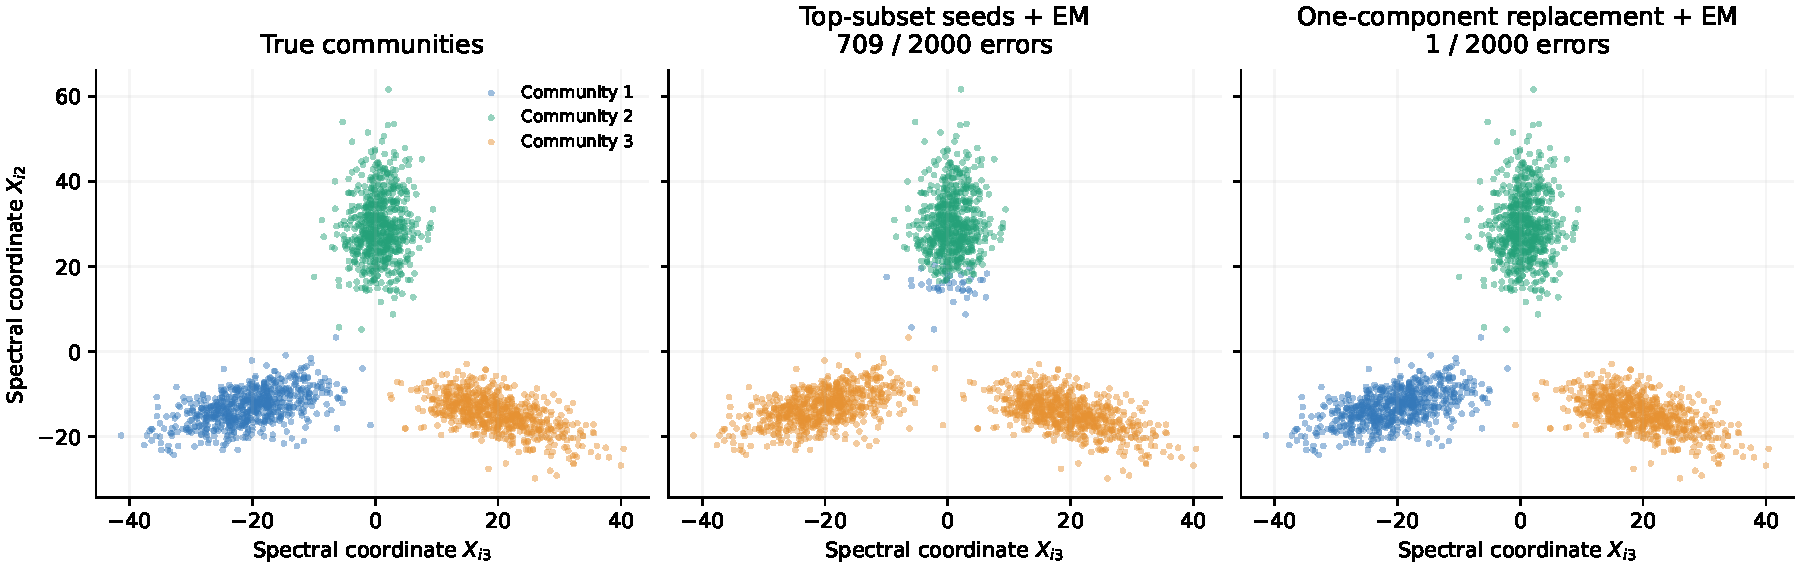
\includegraphics[width=\linewidth]{figures/initialization_failure_repair.pdf}
\caption{The saved design failure, displayed in two coordinates of
$X=\sqrt n U\Lambda$. Left: true communities, used only for evaluation.
Middle: top-subset peeling followed by EM merges the two lower communities
and splits the upper community. Right: an accepted one-component replacement
followed by EM separates the groups and leaves one mislabeled node. Predicted
labels are aligned to truth for display only.}
\label{fig:initialization_repair}
\end{figure}

\subsection{Historical numerical verification and computational scope}

All returned historical profile fits satisfy the declared stopping rule in the 240-graph
comparison. The 120 original peeling errors are reproduced exactly. The
archive contains 6240 EM traces, including replacement proposals, growing
stages, and restart fits, with 27867 recorded trace points. The smallest
observed objective increment is $-1.17\times10^{-10}$, within floating-point
rounding; no increment below $-10^{-7}$ occurs. All 240 selected ten-start
solutions maximize the same final working likelihood within their restart
set. Replacement accepts a likelihood improvement on 22 design graphs and
25 independent graphs, and never lowers the final objective; most of these
small improvements do not change the classification error. Independent
scalar checks reproduce deviance and global-gain calculations with maximum
absolute errors $7.11\times10^{-15}$ and $1.78\times10^{-15}$, respectively.

The present implementation explicitly reconstructs the $n\times n$ profiles
and caches all singleton-candidate scores. Reconstruction costs
$O(n^2K)$, score precomputation costs $O(n^3)$, and storage costs $O(n^2)$.
An EM update costs $O(n^2K)$. A replacement pass tries $K$ additional fits,
whereas ten-start residual seeding uses ten fits. The runs use one numerical
library thread per worker and four worker processes. Python, NumPy, SciPy,
and scikit-learn versions are 3.11.7, 2.1.3, 1.16.2, and 1.7.1. Stored timers
cover all candidate arms and restarts together and exclude graph generation
and eigenpair computation, so they do not support an arm-specific speed
claim. The data sizes $n\le2000$ establish feasibility for this implementation;
candidate-pool approximations and blockwise computations require separate
large-graph validation.

The archived comparisons support improved decoding of a fixed spectrum in
several heterogeneous models and identify a concrete failure of subset
initialization. The new 60-graph study directly evaluates the current
Algorithm~1 and records its weak-signal failures and its lack of a substantive
replacement improvement on that particular collection. Neither collection
estimates an asymptotic error exponent, proves uniform dominance over
$k$-means, or replaces the model assumptions and analysis of
Theorems~\ref{thm:main-recovery} and~\ref{thm:local-spectral-em}.

\paragraph{Companion sparse threshold-certificate checks.}
A separately retained sparse-score implementation tests a uniform-weight
refit together with the replacement trials and accepts only gains of at
least $(\sum_{ij}q_{ij})/\sqrt{\log n}$. Its archived checks contain 24
graphs with $n\in\{256,512\}$, $K\in\{3,4,6\}$, two degree scales,
and two seeds in one heterogeneous assortative family. They record 19 exact
recoveries and seven errors among 9,216 nodes; no natural growing endpoint
requires an accepted replacement in that collection. A separate injected
collapsed population endpoint is repaired in two accepted rounds. These
checks concern the companion sparse threshold rule, not the complete
Bernoulli Algorithm~1. They remain available as
\path{general_k_fresh_checks.json} beside that implementation.

\section{Conclusion}
\label{sec:conclusion}

Spectral compression can preserve the likelihood information needed for nearly optimal community recovery. In a full-rank SBM, the membership subspace contains the block-constant likelihood contrasts. First-order analysis of the empirical adjacency eigenpairs makes this relation quantitative at logarithmic density, and an admissible fixed positive floor preserves the leading Chernoff exponent. The subsequent likelihood and EM analysis controls the dependent whole-graph profiles.

For $K=2$, the original growing likelihood procedure has an end-to-end guarantee. For general fixed $K$, Algorithm~1 supplements the growing fit with $\lceil\log n\rceil$ independent likelihood-residual++ initializations, compares the fitted candidates using the same observed working mixture likelihood, and performs a final EM update before decoding. The resulting recovery bound is
\[
 \mathbb E\,\Mis(\widehat z,z)\le e^{-(1+o(1))I_n}.
\]
Initialization and likelihood selection are part of the proof; weak recovery is not an assumption imposed on an unspecified initializer. The guarantee matches the leading oracle exponent and yields exact recovery above the corresponding logarithmic information threshold.

The paired 240-graph experiments evaluate the original growing and parameter-replacement procedures. They support the usefulness of all-node likelihood gains and likelihood-accepted repairs in resolving severe initialization failures. A full evaluation of the safeguarded combination remains to be carried out. Removing the safeguard while retaining the general fixed-$K$ theorem, establishing calibrated spectral concentration for a lower-density regularizer, and reducing the cost of full profile reconstruction are separate extensions of the completed logarithmic-density theory.

\appendix
\section{Proofs of spectral preservation and statistical results}
\label{app:statistical-proofs}

\subsection{Exact preservation and the population contrast space}

\begin{proof}[Proof of Proposition~\ref{prop:exact-preservation}]
Since $AU=U\Lambda$, multiplication by $U^\top$ gives
$A\Pi=AUU^\top=U\Lambda U^\top=\widetilde A$.  Therefore
$\widetilde A_iw-A_iw=A_i(\Pi-\mathrm{Id})w$.  If $w\in\operatorname{col}(U)$,
then $\Pi w=w$ and the difference vanishes.

Let $N=Z^\top Z=\operatorname{diag}(n_1,\ldots,n_K)$, which is
nonsingular since all communities are nonempty.  The columns of
$ZN^{-1/2}$ are orthonormal, and
\[
 ZPZ^\top=(ZN^{-1/2})(N^{1/2}PN^{1/2})(ZN^{-1/2})^\top.
\]
Nonsingularity of $P$ makes the central matrix nonsingular.  Hence
$ZPZ^\top$ has rank $K$ and column space $\operatorname{col}(Z)$.
For each contrast, define
$\xi_c^{ab}=\log\{P_{ac}(1-P_{bc})/[P_{bc}(1-P_{ac})]\}$.
Then $w^{ab}=Z\xi^{ab}$, which proves membership in that space.
Finally, subtracting $\operatorname{diag}(P_{z_i z_i})$ from $ZPZ^\top$
gives the actual no-self-loop mean, so no rank assertion about that
corrected matrix is needed.
\end{proof}

Full rank cannot be replaced by distinct block rows without a further
contrast-span condition.  For example, let $P=(\log n/n)ss^\top$ for a positive,
nonconstant vector $s$.  Its signal space is spanned by $Zs$, whereas
the sparse log-probability contrast between communities $a,b$ is
$\log(s_a/s_b)\mathbf1$.  When $s_a\ne s_b$, this constant vector does
not belong to $\operatorname{span}(Zs)$.  A rank-one signal projection
does not preserve that contrast by the preceding identity.  This example
only concerns projection onto the population rank-one space; it is not
an impossibility claim for every statistic computed from one empirical
eigenvector.

\subsection{The sparse likelihood correction}

\begin{proof}[Proof of Lemma~\ref{lem:sparse-expansion}]
Write $p_{aj}=P_{a,z_j}$ and $p_{bj}=P_{b,z_j}$ for
$j\ne i$.  The exact binary Bernoulli log-likelihood ratio is
\[
 L_i^{ab}=\sum_{j\ne i}A_{ij}\log\frac{p_{aj}}{p_{bj}}
 +\sum_{j\ne i}A_{ij}\log\frac{1-p_{bj}}{1-p_{aj}}
 +\sum_{j\ne i}\log\frac{1-p_{aj}}{1-p_{bj}}.
\]
For $0\le x\le1/2$, the power series for $\log(1-x)$ implies
$|\log(1-x)+x|\le Cx^2$.  Since
$p_{aj},p_{bj}\le b_+\log n/n$, it also implies
$|\log((1-p_{bj})/(1-p_{aj}))|\le C\log n/n$ and
\[
 \left|\log\frac{1-p_{aj}}{1-p_{bj}}+(p_{aj}-p_{bj})\right|
 \le C(\log n)^2/n^2.
\]
The first term is unchanged in the sparse score, and the final term is replaced by its first-order nonedge offset.
Summing the two displayed remainders proves \eqref{eq:sparse-expansion-error}.

Under any true community, $\deg(i)$ is a sum of independent Bernoulli
variables with mean at most $b_+\log n$.  For $D>b_+$, exponential Markov
inequality with $t=\log(D/b_+)$ and the bound
$\log\mathbb E e^{t\deg(i)}\le b_+\log n(e^t-1)$ give
\[
 \Pr\{\deg(i)>D\log n\}
 \le\exp\{-\log n[D\log(D/b_+)-D+b_+]\}.
\]
The bracket tends to infinity with $D$, so $D_H$ can be chosen for any
$H$.  On the complementary event the correction is at most
$C(D_H+1)(\log n)^2/n=o(1)$.
\end{proof}

\subsection{Chernoff information and the oracle exponent}

\begin{proof}[Proof of Lemma~\ref{lem:oracle-exponent}]
Let $f_a,f_b$ denote the product Bernoulli mass functions of the
incident-edge row in the two hypotheses.  Define
\begin{align*}
 D_\alpha(p_{a,-i}\Vert p_{b,-i})
 &=-\log\sum_x f_a(x)^{1-\alpha}f_b(x)^\alpha\\
 &=-\sum_{j\ne i}\log\big\{p_{aj}^{1-\alpha}p_{bj}^\alpha
                    +(1-p_{aj})^{1-\alpha}(1-p_{bj})^\alpha\big\},\\
 D^*_{i,ab}&=\max_{0\le \alpha\le1}D_\alpha(p_{a,-i}\Vert p_{b,-i}).
\end{align*}
Uniformly for $\alpha\in[0,1]$ and
$u,v\in[b_-\log n/n,b_+\log n/n]$,
\[
 u^{1-\alpha}v^\alpha+(1-u)^{1-\alpha}(1-v)^\alpha
 =1-\{(1-\alpha)u+\alpha v-u^{1-\alpha}v^\alpha\}
   +O((\log n)^2/n^2).
\]
For example, the nonedge product expansion follows by writing it as
$\exp\{(1-\alpha)\log(1-u)+\alpha\log(1-v)\}$;
the first and second derivatives of the nonedge factors are uniformly
bounded for $u,v\le1/2$. Expanding $-\log(1-x)$ and summing gives
\begin{equation}
 D^*_{i,ab}
 =n\max_{0\le \alpha\le1}\sum_c\pi_{c,n}
  \{(1-\alpha)P_{ac}+\alpha P_{bc}-P_{ac}^{1-\alpha}P_{bc}^\alpha\}
  +O((\log n)^2/n+\log n/n),\label{eq:chernoff-expansion}
\end{equation}
where $\pi_{c,n}=n_c/n$. The $O(\log n/n)$ term accounts for the
excluded node. Since $(n/\log n)P$ is fixed and $\pi_{c,n}\to\pi_c>0$,
the displayed expression divided by $\log n$ has a finite limit.
Distinct normalized block rows make this limit positive: taking
$\alpha=1/2$ gives one half the positive weighted sum of the squared
differences of their square roots. Thus $D^*_{i,ab}\asymp \log n$
uniformly over the finitely many pairs and excluded nodes, and
$I_n\asymp \log n$.

The equal-prior Bayes risk is
$R_{i,ab}^{\mathrm{or}}=\frac12\sum_x\min\{f_a(x),f_b(x)\}$.
Since $\min\{u,v\}\le u^{1-\alpha}v^\alpha$,
\begin{equation}
 R_{i,ab}^{\mathrm{or}}\le\tfrac12e^{-D^*_{i,ab}}.
 \label{eq:oracle-upper}
\end{equation}
For completeness, a logarithmic lower bound follows by exponential
tilting, without invoking any refined rate formula.  Let $\alpha_*$ maximize
$D_\alpha(p_{a,-i}\Vert p_{b,-i})$ and set
\[
 f_*(x)=e^{D^*_{i,ab}}f_a(x)^{1-\alpha_*}f_b(x)^{\alpha_*},
 \qquad L(x)=\log\frac{f_a(x)}{f_b(x)}.
\]
All masses are positive, the two distributions differ, and the endpoint
derivatives have opposite signs.  Thus $\alpha_*\in(0,1)$, and differentiating
the normalization gives $\mathbb E_*L=0$.  The tilted incident edges
remain independent, with probabilities
\[
 p_{*,j}=
 \frac{p_{aj}^{1-\alpha_*}p_{bj}^{\alpha_*}}
 {p_{aj}^{1-\alpha_*}p_{bj}^{\alpha_*}+(1-p_{aj})^{1-\alpha_*}(1-p_{bj})^{\alpha_*}}
 \le C\log n/n.
\]
The coefficient of each edge in $L$ is bounded by a constant depending
only on $b_-,b_+$; hence $\operatorname{Var}_*(L)\le C\log n$.
Taking $h_n=(\log n)^{2/3}$, Chebyshev's inequality gives
$\Pr_*(|L|\le h_n)=1-o(1)$.  The change of measure yields
\begin{align*}
 R_{i,ab}^{\mathrm{or}}
 &=\tfrac12e^{-D^*_{i,ab}}
   \mathbb E_*\min\{e^{\alpha_*L},e^{-(1-\alpha_*)L}\}\\
 &\ge\tfrac12e^{-D^*_{i,ab}-h_n}\Pr_*(|L|\le h_n).
\end{align*}
Combining this with \eqref{eq:oracle-upper} proves
$\log R_{i,ab}^{\mathrm{or}}=-D^*_{i,ab}+o(\log n)$, and hence
\eqref{eq:oracle-risk}.  For priors $\nu,1-\nu$ bounded away from zero,
$\min\{\nu f_a,(1-\nu)f_b\}$ is bounded above and below by constant
multiples of $\min\{f_a,f_b\}$, so its leading exponent is unchanged.
\end{proof}

\subsection{Transfer of the leading exponent}

\begin{proof}[Proof of Theorem~\ref{thm:exponent-transfer}]
Suppose the true label of node $i$ is $a$.  If $G_i$ occurs and the
classifier prefers $b\ne a$, then
$\widehat\ell_i(a)-\widehat\ell_i(b)\le0$, and consequently
$L_i^{ab}\le\tau_n$.  For every $\alpha\in[0,1]$,
\[
 \Pr_a\{L_i^{ab}\le\tau_n\}
 \le e^{\alpha\tau_n}\mathbb E_a e^{-\alpha L_i^{ab}}
 =\exp\{\alpha\tau_n-D_\alpha(p_{a,-i}\Vert p_{b,-i})\}.
\]
Selecting a Chernoff maximizer and using $\alpha\le1$ gives
\[
 \Pr\{\widehat z_i\ne z_i\}
 \le\delta_n+\sum_{b\ne a}\exp\{\tau_n-D^*_{i,ab}\}
 \le\delta_n+(K-1)\exp\{-I_n+o(\log n)\}.
\]
Since $I_n\asymp \log n$, we have $o(\log n)=o(I_n)$, and
\eqref{eq:transfer-tail} makes the first term no larger in leading
exponential order.  Averaging over nodes and using that the
permutation-invariant error is no larger than the error under any one
common alignment proves \eqref{eq:conditional-rate}.

The expected number of errors under that alignment is at most
$n\exp\{-(1+o(1))I_n\}$. If
$\liminf_{n\to\infty}I_n/\log n>1$, Markov's inequality gives vanishing
probability of even one error, which proves the exact recovery assertion.
No conclusion when $I_n/\log n\to1$ follows from this argument.
\end{proof}

The matching binary lower bound mentioned after the theorem has a direct
decision-theoretic justification.  Conditional on all other labels, the
rest of the graph is independent of the incident-edge row and has the
same distribution under $a$ and $b$.  Revealing the other labels and
true parameters cannot increase the Bayes risk.  A function of the
graph's spectral summary is also a function of the full graph; its risk
in that binary experiment is therefore at least
$R_{i,ab}^{\mathrm{or}}$.  This argument does not, by itself, assert a
global minimax lower bound over an unspecified parameter space.


\subsection{Full-graph reconstruction and local empirical EM}
\label{app:local-em}

\begin{proof}[Proof of Lemma~\ref{lem:full-spectral}]
The true no-self-loop mean $\E[A\mid z]$ leaves $\operatorname{col}(Z)$ invariant. In the orthonormal membership basis $ZN^{-1/2}$ its restriction is
$N^{1/2}PN^{1/2}-\operatorname{diag}(P_{11},\ldots,P_{KK})$.
Nonsingularity of the fixed matrix $(n/\log n)P$ and positive limiting proportions imply that its $K$ eigenvalues have absolute values between $\kappa_0\log n$ and $C \log n$ for some $\kappa_0>0$ and all large $n$. On the orthogonal complement, the eigenvalues are $-P_{aa}=O(\log n/n)$. Let $U_*$ and $\Lambda_*$ contain these $K$ signal eigenpairs; then
$U_*U_*^\top=\Pi_*$ and $\|U_*\|_{2\to\infty}=O(n^{-1/2})$.

Here $\|M\|_{2\to\infty}=\max_i\|M_i\|_2$. We spell out how the cited entrywise theorem applies. Fix any desired polynomial confidence power. Lei--Rinaldo's spectral norm theorem~\citep[Theorem 5.2]{leirinaldo2015}, with its confidence power chosen arbitrarily large, gives $\|A-\E[A\mid z]\|_{\mathrm{op}}\le C_H\sqrt{\log n}$ outside $O(n^{-H})$. Its upper degree parameter can be taken as $\max\{1,b_+\}\log n$. The signal separation is of order $\log n$, and the eigenvalue condition number is bounded. In the notation of Abbe et al.~\citep[Theorem 2.1]{abbe2020}, take $\gamma=C_H/\sqrt{\log n}$. Their incoherence assumption holds because $\|\E[A\mid z]\|_{2\to\infty}=O(\log n/\sqrt n)$; their row/column independence assumption follows from the independent upper-triangular edges.

For row concentration, their Bernoulli Lemma 7 applies with upper probability $b_+\log n/n$. Choosing its tail parameter large enough gives row failure $O(n^{-H-2})$. For matrices with a fixed number of columns, applying it to the columns and using monotonicity of $\varphi_H$ and of $\varphi_H(x)/x$ to replace the column norms by the Frobenius and maximum-row norms gives the required function
$\varphi_H(x)=C_H/(1\vee\log(1/x))$ for $x>0$, with $\varphi_H(0)=0$.
The constants absorb the fixed number of columns and the ratio of the signal gap to $\log n$. This function is continuous and nondecreasing, $\varphi_H(x)/x$ is nonincreasing, and both $\gamma$ and $\varphi_H(\gamma)$ tend to zero. Thus the remaining smallness condition in that theorem holds for all sufficiently large $n$.

Apply the theorem separately to the positive and negative signal groups, each a contiguous group of eigenvalues, and concatenate their orthogonal alignments. Repeated eigenvalues within either group cause no difficulty. The theorem allows a non-low-rank mean, so the excluded diagonal has not been silently discarded. The norm event also ensures that the empirical largest-absolute-value eigenpairs are precisely these signal groups. We obtain an orthogonal $R$, $V=UR$, and deterministic $\nu_n\to0$ such that
\[
 \|V\|_{2\to\infty}\le C_H/\sqrt n,\qquad
 \|V-AU_*\Lambda_*^{-1}\|_{2\to\infty}\le\nu_n/\sqrt n.
\]
The same polar alignments satisfy the Davis--Kahan bound
$\|V-U_*\|_{\mathrm{op}}\le C_H/\sqrt{\log n}$.
Put $M=R^\top\Lambda R=V^\top A V$. Since
$\|\E[A\mid z]\|_{\mathrm{op}}=O(\log n)$,
\[
 \|M-\Lambda_*\|_{\mathrm{op}}
 \le\|A-\E[A\mid z]\|_{\mathrm{op}}
   +2\|\E[A\mid z]\|_{\mathrm{op}}\|V-U_*\|_{\mathrm{op}}
 \le C_H\sqrt{\log n}.
\]
A degree union bound, with the degree-tail constant chosen for the same confidence power, gives $\max_i\deg(i)\le C_H\log n$.

Set $E=V-AU_*\Lambda_*^{-1}$. The exact row decomposition is
\[
 (\widetilde A-A\Pi_*)_i
 =E_iMV^\top+
 (AU_*)_i\{\Lambda_*^{-1}MV^\top-U_*^\top\}.
\]
The bracket has operator norm $O((\log n)^{-1/2})$, while
$\|(AU_*)_i\|_2\le\deg(i)\|U_*\|_{2\to\infty}\le C_H\log n/\sqrt n$.
Consequently
\[
 \|\widetilde A-A\Pi_*\|_{2\to\infty}
 \le C_H(\log n\nu_n+\sqrt{\log n})/\sqrt n
 =o(\log n/\sqrt n).
\]
Cauchy--Schwarz yields the required uniform row $\ell_1$ bound. Entrywise clipping is 1-Lipschitz, so the bound also holds for $q-q^0$. Moreover,
$|\widetilde A_{ij}|\le\|U_i\|_2\|\Lambda\|_{\mathrm{op}}\|U_j\|_2
\le C_H\log n/n$, proving the profile upper bound.

For the average approximation, define the block counts
$N_{ic}=\sum_{j:z_j=c}A_{ij}$. Because $c_0\log n/n<P_{ac}$, clipping toward $P_{ac}$ cannot increase the coordinate error:
\[
 \|q_i^0-p_{z_i,*}\|_1
 \le\sum_c|N_{ic}-n_cP_{z_i,c}|.
\]
Let $F$ be the sum on the right over all $i$. Its expectation is at most $Cn\sqrt{\log n}+C\log n$; the latter term accounts for the missing diagonal. Changing one independent edge changes $F$ by at most two. The bounded-differences inequality therefore gives
\[
 \Pr\{F-\E F>n(\log n)^{3/4}\}\le e^{-c (\log n)^{3/2}}.
\]
In logarithmic density this is smaller than any fixed inverse polynomial. Combining this average bound with the uniform $q-q^0$ bound, and enlarging a deterministic vanishing $a_n$, proves all assertions.
\end{proof}

\paragraph{Clipped oracle comparisons.}
For later use, fix a true class $a$ and a competitor $b$. Write
$v_c=\log(P_{ac}/P_{bc})$, $N'_{ic}=\max\{N_{ic},n_cc_0\log n/n\}$, and
\[
 L_{i,\mathrm{clip}}^{ab}
 =\sum_cN'_{ic}v_c-\sum_c n_c(P_{ac}-P_{bc}).
\]
This is a comparison score for the analysis, not a computable oracle supplied to the algorithm. For any $\alpha\in[0,1]$, a coordinate with $v_c\ge0$ has a clipped exponential moment no larger than its unclipped moment. If $v_c<0$, put $\beta=-\alpha v_c\ge0$ and $t_c=n_cc_0\log n/n$. For all sufficiently large $n$, $t_c\le\E_a N_{ic}$, including the excluded self-loop, because $c_0<\min_{a,c}nP_{ac}/\log n$. Jensen's inequality implies
\[
 \E_a e^{\beta\max\{N_{ic},t_c\}}
 \le\E_a e^{\beta N_{ic}}+e^{\beta t_c}
 \le2\E_a e^{\beta N_{ic}}.
\]
The counts over different column blocks are independent for a fixed node. Thus clipping costs at most a factor $2^K$ in the Chernoff moment. A direct binomial moment expansion, including an $O(\log n/n)$ diagonal correction, gives
\[
 \log\E_a e^{-\alpha L_{i,\mathrm{raw}}^{ab}}
 =-D_\alpha(p_{a,-i}\Vert p_{b,-i})+O((\log n)^2/n+\log n/n),
\]
where the raw score replaces $N'_{ic}$ by $N_{ic}$.
For any deterministic $\tau_n=o(\log n)$, exponential Markov inequality at the maximizing $\alpha$ yields
\begin{equation}
 \Pr_a\{L_{i,\mathrm{clip}}^{ab}\le\tau_n\}
 \le2^K\exp\{-D^*_{i,ab}+o(\log n)\}.
 \label{eq:clipped-chernoff}
\end{equation}
The argument controls the error probability directly. It does not assume that clipping changes every rare-row score by $o(\log n)$.

\begin{proof}[Proof of Theorem~\ref{thm:local-spectral-em}]
Choose the confidence power $H>2+\limsup_{n\to\infty}I_n/\log n$ in Lemma~\ref{lem:full-spectral} and work on its event. Constants below may depend on the fixed model and floor but not on the iteration. Suppose a responsibility matrix $R$ has aligned average error at most $\gamma$, with $\gamma$ below a sufficiently small fixed constant. Put
$N_a=\sum_iR_{ia}$ and $\bar q_a=n_a^{-1}\sum_{i:z_i=a}q_i$.
Then $|N_a-n_a|\le n\gamma$ and $N_a\ge\pi_{\min}n/2$, where $\pi_{\min}$ is a fixed lower bound on the community proportions for large $n$. The average-profile bound gives
$\|\bar q_a-p_{a*}\|_1\le C a_n\log n$.
The M-step identity gives, deterministically,
\[
 \|\widehat p_a-\bar q_a\|_1
 \le\frac{\sum_i|R_{ia}-Z_{ia}|\|q_i\|_1}{N_a}
       +\left|\frac{n_a}{N_a}-1\right|\|\bar q_a\|_1
 \le C\gamma \log n.
\]
Hence
\begin{equation}
 \max_a\|\widehat p_a-p_{a*}\|_1
 \le C(\gamma+a_n)\log n,\qquad
 c_0\log n/n\le\widehat p_{aj}\le C_H\log n/n.
 \label{eq:local-profile-fit}
\end{equation}
The logarithm is Lipschitz on this common positive range, so its vector $\ell_1$ error is at most $Cn/\log n$ times the profile error. Since $q_{ij}\le C_H\log n/n$, both the fitted linear contrasts and their offsets differ from the true-profile working contrasts by at most $C(\gamma+a_n)\log n$.
The fitted log-weight ratios are bounded: in the unconstrained update $N_a/n$ is bounded away from zero; for a fixed positive floor this follows directly from feasibility.

Combining the uniform row $q-q^0$ bound with these parameter bounds gives, for every node and pair,
\begin{equation}
 |\widehat\ell_i(a)-\widehat\ell_i(b)-L_{i,\mathrm{clip}}^{ab}|
 \le C(\gamma+a_n)\log n+C.
 \label{eq:local-score-fit}
\end{equation}
No independence of $R$, $q$, and the incident edges has been used. With $\gamma=\gamma_n\to0$, a wrong classification implies
$L_{i,\mathrm{clip}}^{ab}\le o(\log n)$ for some competitor, apart from the initialization or graph exceptional events. Equation~\eqref{eq:clipped-chernoff} and a finite union bound prove the one-update rate.

We also verify that further EM updates remain in the required region. Let
\[
 \kappa=\liminf_n\min_{a\ne b}
 (\log n)^{-1}D(p_{a*}\Vert p_{b*})>0.
\]
Choose a small fixed basin radius $\gamma_0>0$ so that the error bound from \eqref{eq:local-profile-fit} for $\gamma\le\gamma_0$ is less than $\kappa \log n/8$ in each score comparison for large $n$. Also choose a fixed small $t_0>0$ so that a row with
$\|q_i-p_{z_i,*}\|_1\le t_0\log n$ has an observation-contrast error less than $\kappa \log n/8$.
At the population observation $q_i=p_{z_i,*}$, the working margin equals $D(p_{z_i,*}\Vert p_{b*})\ge\kappa \log n/2$ for large $n$. The specified row deviation costs at most $\kappa \log n/8$, and the fitted-parameter and bounded weight corrections together cost at most $\kappa \log n/8$, leaving a correct-class margin of at least $\kappa \log n/4$.
The average-profile bound shows that the remaining rows constitute at most $a_n/t_0$ of all nodes. Thus the next E-step has aligned average responsibility error at most
\[
 b_n=2a_n/t_0+2(K-1)e^{-\kappa \log n/4}\longrightarrow0.
\]
This bound holds uniformly for every $R$ in the fixed basin. Eventually $b_n<\gamma_0$, so the basin is invariant. Starting with error $\gamma_n\to0$, every later responsibility matrix has error at most $\max\{\gamma_n,b_n\}=o(1)$.
Equation~\eqref{eq:local-score-fit} therefore holds with one deterministic $o(\log n)$ bound for every later fitted score on the same event. This includes a data-dependent finite stopping time and needs no union bound over iterations.

Finally add the initialization failure $\delta_n$ and the graph failure $O(n^{-H})$ to the per-node Chernoff bound and average over nodes. Since $H>2+\limsup_{n\to\infty}I_n/\log n$, the graph failure is negligible compared with $e^{-I_n}$, and the assumed initialization reliability preserves the leading exponent. If $\liminf_{n\to\infty}I_n/\log n>1$, multiplying the expected error by $n$ and applying Markov's inequality gives exact recovery with probability tending to one.
\end{proof}

\begin{proof}[Proof of Corollary~\ref{cor:provable-warmstart}]
The spectral norm and Davis--Kahan bounds above give an orthogonal alignment with
$\|U-U_*R^\top\|_F^2=O((\log n)^{-1})$ outside $O(n^{-H})$.
The $K$ distinct population row centers have squared separation at least $2/n$, since the rows of $ZN^{-1/2}$ from different groups are orthogonal, with squared norms $1/n_a$ and $1/n_b$.
A fixed-factor approximate $K$-means solution has total squared error at most a constant times $\|U-U_*R^\top\|_F^2$. The deterministic center-matching argument (also used in Lei--Rinaldo's clustering bound) then gives $\Mis(\widetilde z,z)=O((\log n)^{-1})$: the total squared discrepancy of fitted centers from the population rows is $O((\log n)^{-1})$; positive community sizes force one fitted center near each distinct population center; each incorrectly assigned row contributes a constant multiple of $1/n$ to that discrepancy. Hard responsibilities consequently have aligned average error $2\Mis(\widetilde z,z)=O((\log n)^{-1})$.

For a concrete randomized implementation, the $K$-means++ expected squared-error bound is $C_K=8(\log K+2)$ times the optimum~\citep{arthur2007}. Conditional on $U$, Markov's inequality bounds the chance of exceeding $2C_K$ times the optimum by $1/2$ for each independent seeding. Taking at least $(H+2)\log_2 n$ independent seedings and selecting the smallest squared-error potential makes that failure at most $n^{-H-2}$. Any subsequent Lloyd steps can only lower this potential. The zero-optimum case is recovered exactly by the seeding. For fixed $K$ this costs polynomial time and uses only $U$. Choose $H>\limsup_{n\to\infty}I_n/\log n$, combine this event with the spectral event, and apply Theorem~\ref{thm:local-spectral-em}.
\end{proof}


\subsection{End-to-end likelihood initialization}
\label{app:end-to-end}

\paragraph{Proof of Theorem~\ref{thm:two-community-growing}.}
Fix $H>2+\limsup_{n\to\infty}I_n/\log n$ and work on the event of Lemma~\ref{lem:full-spectral}. All constants below may depend on $H$ and the fixed model. Enlarge its deterministic $a_n\to0$ if necessary to bound both displayed profile errors. Put $\pi_{a,n}=n_a/n$,
\[
 m_b=\sum_{a=1}^2\pi_{a,n}P_{ab},\qquad
 D_{\pi_n}(x\Vert y)=
 \sum_b\pi_{b,n}\{x_b\log(x_b/y_b)-x_b+y_b\}.
\]
The block values of $q_c^0$ are
\[
 v_{cb}=\max\left\{\frac{\sum_{j:z_j=b}A_{cj}}{n_b},
                         \frac{c_0\log n}{n}\right\},
 \qquad q_{cj}^0=v_{c,z_j}.
\]
This is only an analysis variable. In particular $v_c$ may be a rare extreme candidate, and we do not assume it is near its own community profile. Let
\[
 h_a(v)=\frac{n}{\log n}\sum_b\pi_{b,n}
 \{P_{ab}\log(v_b/m_b)-(v_b-m_b)\},\qquad
 \Phi_n(v)=\sum_a\pi_{a,n}[h_a(v)]_+.
\]
The global profile mean $\overline q$ differs from $(m_{z_j})_{j=1}^n$ in $\ell_1$ norm by at most $a_n\log n$. The uniform bound on $q_c-q_c^0$ and the common positive box give
\[
 \left|[\ell_i(q_c)-\ell_i(\overline q)]-\log nh_{z_i}(v_c)\right|
 \le C\{\|q_i-p_{z_i,*}\|_1+a_n\log n\}.
\]
Here the parameter perturbation costs
$C\|q_c-q_c^0\|_1+C\|\overline q-(m_{z_j})_{j=1}^n\|_1$,
because $q_{ij}\le C \log n/n$ and $\log$ is $n/(c_0\log n)$-Lipschitz. The remaining observation perturbation multiplies a uniformly bounded log ratio. Since positive part is 1-Lipschitz, summing yields the simultaneous candidate bound
\[
 \sup_c\left|\frac{\Delta_2(c)}{n\log n}-\Phi_n(v_c)\right|\le Ca_n.
\]
Every true class has a candidate with $\|q_c-p_{a*}\|_1=o(\log n)$ by the average error bound and its positive proportion. The same is true of $q_c^0$, so
$(n/\log n)\sum_b\pi_{b,n}|v_{cb}-P_{ab}|=o(1)$.
The fixed normalized matrix and positive limiting proportions imply that
\[
 g_0=\lim_{n\to\infty}\max_a
 \frac{n\pi_{a,n}}{\log n}
 D_{\pi_n}\big((P_{ab})_{b=1}^2\Vert m\big)>0.
\]
Positivity follows because the two distinct normalized block rows cannot both equal their mean. Continuity on the normalized common positive box and the candidate bound imply that the selected candidate satisfies $\Phi_n(v_c)\ge g_0/2$ for large $n$.

The decisive two-class identity is
\[
 \sum_a\pi_{a,n}h_a(v)=-\frac{n}{\log n}D_{\pi_n}(m\Vert v)\le0.
\]
Together with $\Phi_n(v_c)\ge g_0/2$, it forces exactly one of $h_1(v_c),h_2(v_c)$ to be positive. Moreover
\[
 h_{\rm pos}(v_c)\ge g_0/2,\qquad
 h_{\rm neg}(v_c)\le-g_0/2,
\]
since each weighted positive or negative magnitude is at least $g_0/2$ and each proportion is at most one. The initial two mixture weights are equal, so they do not alter this score comparison.

Take $\tau_n=\sqrt{a_n}+(\log n)^{-1}$. At most $(a_n/\tau_n)n=o(n)$ observations have $\|q_i-p_{z_i,*}\|_1>\tau_n\log n$. Every other observation has the correct initial component margin at least $g_0\log n/4$ after the above score perturbations. After a common label alignment, the first E-step therefore satisfies
\[
 \frac1n\sum_{i,a}|R_{ia}-Z_{ia}|
 \le \frac{2a_n}{\tau_n}+2e^{-g_0\log n/4}=o(1).
\]
The graph event has failure $O(n^{-H})$, so these responsibilities meet the reliability condition in Theorem~\ref{thm:local-spectral-em}. The evaluated fitting loop always performs its first M-step before it may stop. That theorem gives the claimed exponent for the first resulting decode and all subsequent finite updates, including the evaluated stopping rule. Its exact-recovery implication also applies. \qed

\paragraph{Proof of Theorem~\ref{thm:certified-likelihood}.}
Again choose a fixed $H>2+\limsup_{n\to\infty}I_n/\log n$ and condition on the event in Lemma~\ref{lem:full-spectral}. Let $a_n\to0$ bound its average profile error, and write $c_0\log n/n\le q_{ij}\le C_H\log n/n$. True profiles have the same positive box after enlarging $C_H$. Full rank implies distinct block rows; their limiting positive proportions give constants $\kappa,s>0$ such that
\[
 \min_{a\ne b}D(p_{a*}\Vert p_{b*})\ge\kappa \log n,\qquad
 \min_{a\ne b}\|p_{a*}-p_{b*}\|_1\ge s\log n
\]
for all sufficiently large $n$.

\emph{Reliable seed coverage.}
On this box the two derivatives of the scalar deviance are $\log(x/y)$ and $1-x/y$, which are uniformly bounded. Consequently
\[
 \begin{split}
 0\le D(x\Vert y)&\le C\log n,\\
 |D(x\Vert y)-D(x'\Vert y')|
 &\le C(\|x-x'\|_1+\|y-y'\|_1).
 \end{split}
\]
Set $\tau_n=\sqrt{a_n}+(\log n)^{-1}$. Call row $i$ good when $\|q_i-p_{z_i,*}\|_1\le\tau_n\log n$; the remaining rows number at most $(a_n/\tau_n)n$. Conditional on previously selected seeds being good and representing distinct classes, every good row in a represented class has residual at most $2C\tau_n\log n$. Every good row in an unrepresented class has residual at least $\kappa \log n/2$, by the Lipschitz bound. Before $K$ seeds have been selected, an unrepresented class supplies at least $\pi_{\min}n/2$ good rows. Hence total sampling mass is at least $cn\log n$, whereas the mass of represented good rows and all bad rows is at most
\[
 C(\tau_n+a_n/\tau_n)n\log n.
\]
The first uniform seed is bad with probability at most $a_n/\tau_n$. A union bound over the fixed $K$ choices gives single-run failure at most
\[
 r_{H,n}\le C_K(\tau_n+a_n/\tau_n)=o(1).
\]
The all-zero fallback cannot occur on this successful path while a class remains unrepresented. Conditional on $q$, the restart streams are independent. Their joint failure probability is at most
\[
 r_{H,n}^{\lceil\log n\rceil}=n^{-\omega(1)}.
\]
This amplification requires no knowledge of $H$ or the separation constants.

\emph{Likelihood selection certifies the winning fit.}
Define the observation-only saturation constant and soft deviance
\[
 S_q=\sum_{i,j}(q_{ij}\log q_{ij}-q_{ij}),\qquad
 F(\widehat\pi,\widehat p)=
 -\sum_i\log\sum_k\widehat\pi_k
       e^{-D(q_i\Vert\widehat p_{k*})}.
\]
There is the exact identity
\[
 \mathcal L=S_q-F,\qquad
 F\ge\sum_i\min_kD(q_i\Vert\widehat p_{k*})\ge0.
\]
Observation Gamma terms, if restored, are common to every fit. A successful run starts with one good seed for each class and uniform weights. Thus
\[
 F_{\rm initial}
 \le C(a_n+\tau_n)n\log n+n\log K
 =:\epsilon_nn\log n,\qquad \epsilon_n\to0.
\]
Every exact EM update increases $\mathcal L$ and decreases $F$. Selecting the largest final $\mathcal L$ across all runs, including the growing endpoint, therefore gives
\[
 F_{\rm selected}\le\epsilon_nn\log n.
\]
This argument does not require identifying the successful run, fitting any run to stationarity, or proving anything about the growing branch's basin dynamics.

All candidate means remain in the same box, since they start at rows or the global mean of $q$ and each M-step forms a convex combination. Keeping the previous mean in a zero-mass component preserves the box too. Strong convexity of $x\log x-x$ on the box, followed by Cauchy--Schwarz, gives
\[
 D(x\Vert y)
 \ge\frac{n\|x-y\|_2^2}{2C_H\log n}
 \ge\frac{\|x-y\|_1^2}{2C_H\log n}.
\]
Consequently
\[
 \sum_i\min_k\|q_i-\widehat p_{k*}\|_1^2
 \le 2C_H\epsilon_nn(\log n)^2.
\]
Put $\eta_n=\sqrt{a_n}+\epsilon_n^{1/4}+(\log n)^{-1}$. The fractions of rows farther than $\eta_n\log n$ from their true profile, or from every fitted profile, are at most $a_n/\eta_n$ and $2C_H\epsilon_n/\eta_n^2$, respectively; both tend to zero. Each positive-proportion true class has a row avoiding both bad sets. Its fitted center is within $2\eta_n\log n$ of its true center. The separation $s\log n$ forces different classes to use different fitted centers; with exactly $K$ centers this gives a single label permutation satisfying
\[
 \max_a\|\widehat p_{a*}-p_{a*}\|_1\le2\eta_n\log n.
\]

\emph{The selected responsibilities are weakly consistent.}
For a row with $\|q_i-p_{z_i,*}\|_1\le\eta_n\log n$, every wrongly matched center is at $\ell_1$ distance at least $s\log n/2$ for large $n$, hence its deviance is at least
$c_*\log n$, with $c_*=s^2/(8C_H)>0$.
For the selected fit's exact E-step, write
\[
 R_{ik}=
 \frac{\widehat\pi_k e^{-D(q_i\Vert\widehat p_{k*})}}
 {\sum_l\widehat\pi_l e^{-D(q_i\Vert\widehat p_{l*})}}.
\]
The variational identity is
\[
 -\log\sum_k\widehat\pi_k e^{-D_{ik}}
 =\sum_kR_{ik}D_{ik}
   +\operatorname{KL}(R_i\Vert\widehat\pi)
 \ge\sum_kR_{ik}D_{ik}.
\]
Summing over the typical rows and bounding each remaining row's responsibility error by two gives
\[
 \frac1n\sum_{i,k}|R_{ik}-Z_{ik}|
 \le\frac{2a_n}{\eta_n}+\frac{2\epsilon_n}{c_*}
 =:\gamma_n\longrightarrow0
\]
after the above permutation. The identity remains valid with zero weights using the usual zero-mass conventions, and also with a feasible fixed weight floor.

This weak-start conclusion fails only if the graph event fails or every restart fails, a probability at most $O(n^{-H})+n^{-\omega(1)}$. Apply Theorem~\ref{thm:local-spectral-em} to the mandatory final M-step. Since $H>2+\limsup_{n\to\infty}I_n/\log n$, the initialization failures are negligible at the target exponent scale. This proves the complete decoder's expected-error bound and its exact-recovery consequence. Prescribed polynomial EM iteration limits and $\lceil\log n\rceil$ restarts give polynomial computational cost. \qed

\subsection{Row-independent projection errors}

\begin{proof}[Proof of Theorem~\ref{thm:independent-projection}]
Condition on the data generating $\Pi_i$ and on $H_i$.  Work in the
$n-1$ coordinates other than $i$, and write $\Pi_*=\Pi_{*,i}$,
$\Pi=\Pi_i$, $w=w_{-i}^{ab}$, $p_j=\mathbb E A_{ij}$, and
$e=(\Pi-\mathrm{Id})w$.  The fixed block assumptions imply
\[
 w\in\operatorname{col}(\Pi_*),\quad
 p\in\operatorname{col}(\Pi_*),\quad
 \|w\|_2\le C\sqrt n,\quad \|w\|_\infty\le C,
 \quad \|p\|_2\le C\log n/\sqrt n.
\]
The constants are uniform over the finitely many contrasts and true
labels.  For orthogonal projectors,
\[
 \|\Pi_*(\mathrm{Id}-\Pi)\Pi_*\|_{\mathrm{op}}
 =\|(\mathrm{Id}-\Pi)\Pi_*\|_{\mathrm{op}}^2\le\eta_n^2,
\]
because the left matrix is
$[(\mathrm{Id}-\Pi)\Pi_*]^\top[(\mathrm{Id}-\Pi)\Pi_*]$.  It follows that the mean projection
error has the quadratic bound
\begin{equation}
 |p^\top e|
 \le\|p\|_2\|w\|_2\eta_n^2
 \le C\log n\eta_n^2.\label{eq:quadratic-bias}
\end{equation}
Also,
$\|e\|_2\le C\sqrt n\eta_n$.  By Cauchy--Schwarz and projector
leverage,
\[
 |(\Pi w)_j|\le\|\Pi\mathbf e_j\|_2\|w\|_2
 =\sqrt{\Pi_{jj}}\|w\|_2\le C\sqrt L,
\]
so $\|e\|_\infty\le M$ for a fixed positive constant $M$.

Conditional independence makes
$X_j=(A_{ij}-p_j)e_j$ independent and centered.  They satisfy
$|X_j|\le M$ and
\begin{equation}
 V=\sum_j\mathbb E X_j^2
 \le b_+\log n/n\|e\|_2^2\le C\log n\eta_n^2.
 \label{eq:projection-variance}
\end{equation}
Here a Bennett bound is stronger than the simpler Bernstein bound at
the required scale.  We include its short derivation.  For a centered
$X$ with $|X|\le M$ and $\lambda\ge0$, Taylor expansion and
$|X|^k\le M^{k-2}X^2$ imply
\[
 \mathbb E e^{\lambda X}
 \le1+\frac{\mathbb E X^2}{M^2}
                (e^{\lambda M}-1-\lambda M).
\]
After multiplying moment-generating functions and using $\log(1+x)\le x$,
exponential Markov inequality optimized in $\lambda$ gives
\begin{equation}
 \Pr\{|\textstyle\sum_jX_j|>t\mid \Pi\}
 \le2\exp\left\{-\frac{V}{M^2}
 h\left(\frac{Mt}{V}\right)\right\},\qquad
 h(u)=(1+u)\log(1+u)-u,\label{eq:bennett}
\end{equation}
with the evident interpretation when $V=0$.

To choose a uniform vanishing error scale, put
$a_n=\max\{\eta_n^2,e^{-\log n}\}$,
$s_n=\log(1/a_n)$.
Both $a_n\to0$ and $s_n\to\infty$.  Take $t=\log n/\sqrt{s_n}$.
The bound \eqref{eq:bennett} remains valid with $V$ replaced by the
upper bound $C\log na_n$, since its exponent is nonincreasing in the
variance argument.  As $u\to\infty$, $h(u)\sim u\log u$, so
\[
 \frac{C\log na_n}{M^2}
 h\left(\frac{M}{Ca_n\sqrt{s_n}}\right)
 =\frac{\log n}{M\sqrt{s_n}}
   \{s_n-\tfrac12\log s_n+O(1)\}(1+o(1))
 \ge c \log n\sqrt{s_n}
\]
for all sufficiently large $n$.  Combining this with
\eqref{eq:quadratic-bias} gives, for
$\tau_n=\log n/\sqrt{s_n}+C\log n\eta_n^2=o(\log n)$,
\[
 \Pr\{|A_{i,-i}(\Pi-\mathrm{Id})w|>\tau_n\mid \Pi,H_i\}
 \le2e^{-c \log n\sqrt{s_n}}.
\]
Union bound over the finitely many contrasts and addition of
$\Pr(H_i^c)$ prove \eqref{eq:independent-projection-tail} with
$h_n=c\sqrt{s_n}\to\infty$.  The last claim is an application of
Theorem~\ref{thm:exponent-transfer}.
\end{proof}

\section{Proofs of initialization and optimization properties}
\label{app:optimization-proofs}

\subsection{Frozen-candidate greedy gains}

\begin{proposition}[Greedy gain guarantee]
\label{prop:greedy-gain}
Let $s_{ic}$ be fixed finite candidate scores and let $S_0$ be a fixed
nonempty seed set.  For candidate sets $T$, define
\[
 G(T)=\sum_i\max_{c\in S_0\cup T}s_{ic}
      -\sum_i\max_{c\in S_0}s_{ic}.
\]
Then $G$ is normalized, monotone, and submodular.  If $m\ge1$ greedy
steps select a set $T_m$ and $T^*$ maximizes $G$ over sets of at most
$m$ candidates, then
\[
 G(T_m)\ge\{1-(1-1/m)^m\}G(T^*)\ge(1-e^{-1})G(T^*).
\]
\end{proposition}

\begin{proof}
Normalization and monotonicity follow immediately from the definition.
The marginal gain of candidate $c$ is
\[
 G(T\cup\{c\})-G(T)
 =\sum_i\left(s_{ic}-\max_{b\in S_0\cup T}s_{ib}\right)_+.
\]
If $T\subseteq T'$, each maximum in the right side increases, so the
marginal gain decreases.  This proves submodularity.
For the greedy set $T_t$ at time $t$, monotonicity and telescoping
diminishing returns give
\begin{align*}
 G(T^*)-G(T_t)
 &\le G(T_t\cup T^*)-G(T_t)\\
 &\le\sum_{c\in T^*\setminus T_t}
        \{G(T_t\cup\{c\})-G(T_t)\}\\
 &\le m\{G(T_{t+1})-G(T_t)\}.
\end{align*}
Starting from $G(T_0)=0$ and iterating this inequality proves the
claimed factor.  The final inequality follows from
$(1-1/m)^m\le e^{-1}$, including the case $m=1$.
\end{proof}

This is the standard cardinality-constrained submodular greedy
guarantee~\cite{nemhauser1978}.  It controls added explanation relative
to the fixed initial seed, not the multiplicative approximation of a
possibly negative total log score.  It does not apply unchanged when
intermediate EM steps alter the candidate scores.

\subsection{Noiseless profile selection}

\begin{proposition}[Population profile selection]
\label{prop:noiseless-seeding}
Suppose $q_i=\theta_{z_i}$, where the $K$ positive profile vectors
$\theta_1,\ldots,\theta_K$ are pairwise distinct and every class is
nonempty.  The candidate pool consists of these node profiles.  From
any first seed belonging to this candidate pool, $K-1$ subsequent global-gain greedy steps select all
$K$ different profiles.  Maximum working-score classification using
those profiles recovers $z$ up to permutation.
\end{proposition}

\begin{proof}
For $x,\widehat p>0$ coordinatewise, write
$\ell_x(\widehat p)=\sum_jx_j\log\widehat p_j-\sum_j\widehat p_j$.  Then
\[
 \ell_x(x)-\ell_x(\widehat p)
 =\sum_j\{x_j\log(x_j/\widehat p_j)-x_j+\widehat p_j\}
 =D(x\Vert\widehat p)\ge0,
\]
with equality precisely when $x=\widehat p$; the inequality follows from
$\log u\le u-1$.  If a profile has already been selected, selecting a
duplicate has zero gain.  If profile $\theta_b$ has not been selected,
then each node in class $b$ gains
$\min_{a\in S}D(\theta_b\Vert\theta_a)>0$
when it is added.  Therefore some unselected profile has strictly
positive gain, and greedy cannot select a duplicate before all distinct
profiles have been selected.  The same strict divergence inequality
makes each node's own profile its unique best score after selection.
\end{proof}

The proposition concerns the frozen node-profile selection control in an abstract noiseless profile model. It does not directly cover Algorithm~1, whose initial mean need not be a node profile and whose intermediate EM fits change the parameters.  It does
not replace a stability analysis for random spectral profiles, and it
does not erase the diagonal distinction in a no-self-loop SBM.

\subsection{Exact working EM and accepted replacements}

\begin{proposition}[Objective convergence of exact working EM]
\label{prop:em-monotonicity}
For fixed strictly positive profiles $q_1,\ldots,q_n$, let
\[
 \mathcal L(\widehat\pi,\widehat p)=\sum_i\log\sum_{a=1}^K
       \widehat\pi_a\exp\{\ell_i(\widehat p_a)\},\qquad
 \ell_i(\widehat p_a)=\sum_jq_{ij}\log\widehat p_{aj}-\sum_j\widehat p_{aj}.
\]
Starting with positive parameters and positive mixture weights, the
exact E-step and unconstrained exact M-step
\begin{align*}
 r_{ia}&=\frac{\widehat\pi_a e^{\ell_i(\widehat p_a)}}
                   {\sum_b\widehat\pi_b e^{\ell_i(\widehat p_b)}},\qquad
 N_a=\sum_i r_{ia},\\
 \widehat\pi_a^{\mathrm{new}}&=N_a/n,\qquad
 \widehat p_{aj}^{\mathrm{new}}=\frac{\sum_i r_{ia}q_{ij}}{N_a}
\end{align*}
make $\mathcal L$ nondecreasing.  Its numerical values converge to a
finite limit.  The same monotonicity statement holds for an exact
M-step maximizing over any stated constraint set containing the current
parameters, and for replacement proposals accepted only when their
final $\mathcal L$ improves.
\end{proposition}

\begin{proof}
For row-wise probability vectors $r_i$, define the variational objective
\[
 \mathcal F(r,\widehat\pi,\widehat p)=
 \sum_{i,a}r_{ia}\{\log\widehat\pi_a+\ell_i(\widehat p_a)-\log r_{ia}\}.
\]
The log-sum inequality gives
$\mathcal F(r,\widehat\pi,\widehat p)\le\mathcal L(\widehat\pi,\widehat p)$, with equality
for the E-step responsibilities.  For fixed $r$, maximizing
$\sum_aN_a\log\widehat\pi_a$ over the simplex gives $\widehat\pi_a=N_a/n$.
For each profile coordinate, maximizing
$(\sum_i r_{ia}q_{ij})\log\widehat p_{aj}-N_a\widehat p_{aj}$ gives the displayed
weighted mean.  These are interior maxima because all inputs and
responsibilities are positive.  Thus the E-step makes the variational
bound tight and the M-step raises it, proving monotonicity.

The saturated-score inequality used in the preceding proof implies
$\ell_i(\widehat p_a)\le\ell_i(q_i)$ for every $i,a$.  Since
$\sum_a\widehat\pi_a=1$,
\[
 \log\sum_a\widehat\pi_a e^{\ell_i(\widehat p_a)}\le\ell_i(q_i).
\]
Consequently $\mathcal L\le\sum_i\ell_i(q_i)<\infty$.
A nondecreasing real sequence bounded above has a finite limit.
For a constrained exact M-step the current parameters remain feasible,
so the same variational argument applies.  The replacement assertion
follows directly from its acceptance rule.
\end{proof}

This proposition proves convergence of objective values.  It proves
neither convergence to the global maximum nor recovery of the true
labels. The implementation uses an exact active-set maximizer on the
floored simplex, so its weight constraint is covered by the constrained
version of this proposition. Its finite stopping tolerance and
floating-point accuracy are assessed separately in Section~\ref{sec:experiments}.

\begin{proposition}[Profile hull and spectral dimension]
\label{prop:profile-hull}
Every responsibility-weighted profile M-step produces a profile in the convex hull of the rows of $q$. If the unmodified reconstruction $q=U\Lambda U^\top$ is used and the resulting means are positive, all fitted profiles lie in its row space, of dimension at most $K$. Entrywise positive clipping can increase this dimension.
\end{proposition}
\begin{proof}
The coefficients $R_{ia}/N_a$ are nonnegative and sum to one, so the update is a row convex combination. Every such combination also lies in the row space. The unmodified reconstruction has rank at most $K$. The clipping operation is nonlinear and has no corresponding rank-preservation identity.
\end{proof}

\section{Implementation and reproducibility}
\label{app:implementation}

\subsection{Current implementation}
The source, complete numerical evidence and compiled manuscript are at
\begin{center}
\url{https://github.com/zhixin0825/spectral-lrt}.
\end{center}
Algorithm~1 is implemented by \texttt{SpectralLikelihood.decode()} in
\begin{center}
\small\path{experiments/20261010_general_density/spectral_likelihood.py}.
\end{center}
It accepts an $n\times K$ eigenvector array and a length-$K$ array of the corresponding signed eigenvalues. The decoder receives neither the adjacency matrix, true labels, true block probabilities nor node degrees. Retaining the top-$|\lambda|$ eigenpairs is the preceding spectral step.

The default \texttt{score\_family='bernoulli'} evaluates \eqref{eq:working-score}. The floor coefficient defaults to $c_0=10^{-4}$; its theoretical guarantee requires the explicit admissibility condition in Section~\ref{sec:algorithm}, not merely positive block probabilities. The spectral scale is $\max\{1,\max_a|\lambda_a|\}$, and the reconstructed entries are clipped on both sides. The original adjacency is not regularized. The optional \texttt{score\_family='sparse'} is a score control on precisely the same $q$, and is not the default general-density algorithm.

Growing uses at most 100 exact M-steps per stage. A fit stops after at least one M-step if hard labels are unchanged and its absolute soft-loss change is at most $10^{-9}n$. Replacement uses at most $\lceil\log n\rceil$ rounds, tries every component deletion against the same incumbent, initializes each trial's weights uniformly, and uses one M-step per trial by default. A full round with no improvement stops the search. This rule is justified by the contraction certificate in Appendix~\ref{app:replacement-proof}. Calling \texttt{decode()} always executes the final E-step and one profile/weight M-step before returning labels.

The implementation uses the unconstrained simplex weight update. Zero-mass components retain their previous profile. Log-sum-exp arithmetic evaluates responsibilities and the soft divergence loss $F$ without exponentiating very negative raw log-likelihoods. Theoretical divergences are nonnegative; the code clips negative floating-point residue at zero. Weighted means, including the initial global mean, are clipped back to the same feasible interval solely to correct roundoff in convex combinations. The theorem is an exact-arithmetic result; recorded numerical checks assess implementation accuracy to floating-point precision.

The user may increase either fitting budget. Explicitly requesting fewer replacement rounds is an experimental option and does not automatically retain the stated general-$K$ initialization guarantee. The proven default budget is $\lceil\log n\rceil$, with valid early stopping after a full unsuccessful round.

\subsection{Current finite-graph and population evidence}
The complete 60-graph design is specified by
\begin{center}
\small\path{experiments/20261010_general_density/benchmark_results/protocol.json}.
\end{center}
It fixes all graph seeds, model families, density settings, method parameters, and hashes of the code used at fitting time. Each graph directory retains the original $A$, $P$, true labels for evaluation, exact retained $(U,\Lambda)$, all fitted profiles and weights, every candidate's hard loss, and full EM objective traces. Ground truth is not used for fitting, selecting replacements, or stopping. The aggregate CSV contains all 360 graph--method combinations.

The archived fitting engine is retained as \texttt{engine\_at\_fitting.py}. A subsequent boundary fix clips the rounded initial mean when a graph has all reconstructed entries at the floor. The maintenance record checks that this expression is bitwise unchanged on every archived graph, so the saved benchmark is unaffected. The original fitting hashes remain in the frozen protocol; maintenance provenance is recorded separately.

The five-community population calculation and the exact rational interval certificate are in
\begin{center}
\small\path{experiments/20261010_general_density/population_audit/}.
\end{center}
They record the positive-definiteness certificate, strict all-node-gain comparisons, the limiting one-update-per-stage trajectory, and replacement trial results. The distinction between a population limiting path, a finite-graph theorem, and fully iterated growing is maintained in the report. The manifest \texttt{SHA256SUMS} identifies the saved numerical records.

\subsection{Historical experiments and entry points}
The earlier 240-graph comparison is preserved at
\path{experiments/20261009_residual_likelihood_seeding/}.
The \texttt{residual\_seed.py} module retains several sparse-score methods, using
\[
 \ell_i^{\mathrm{sparse}}(\widehat p)=\sum_jq_{ij}\log\widehat p_j-\sum_j\widehat p_j.
\]
Its current default \path{method='global_gain_certified'} calls the separate sparse threshold-certificate implementation \texttt{Work.iterative\_certified\_growing()}. It uses an adaptive lower-only floor, a uniform-weight refit of the current centers as well as $K$ replacement trials, acceptance threshold $(\sum_{ij}q_{ij})/\sqrt{\log n}$, and a cap of $\lceil(\log n)^2\rceil$ accepted rounds. Its general-$K$ proof for the sparse range $p\to0$ with $p=\Omega(\log n/n)$ and its 24-graph implementation checks are retained as a companion version. They preceded the complete Bernoulli density extension and direct soft-loss contraction presented here, which allow the full range \eqref{eq:density-condition}.

In that module, \path{method='global_gain'} is the growing-only branch, \path{method='global_gain_restarts'} selects independent residual starts, and \path{method='repair'} is the historical single-pass repair. None identifies the current full-Bernoulli Algorithm~1, whose entry point is specified above. The actual 240-graph runs used the earlier lower floor $10^{-4}\log n/n$ and their recorded protocol, not the adaptive-floor default now present in the companion module. Their profiles were not constrained to lie below one. The preserved benchmark runner explicitly selects \texttt{floor\_mode='historical'} for these original arms; their earlier source is also accessible in repository history.

The archived 240-graph fits use an exact weight M-step with floor $f=10^{-8}$. For a fixed $0\le f<1/K$, it solves
\[
 \max_{\pi_a\ge f,\,\sum_a\pi_a=1}\sum_aN_a\log\pi_a,
 \qquad \pi_a=\max\{f,N_a/\lambda\},
 \quad\sum_a\pi_a=1.
\]
An active-set solver determines $\lambda$; naive clipping and renormalization is not this optimizer. The current main theorem and implementation use $f=0$.

Historical fits stop only when labels are unchanged, relative profile and absolute weight changes are at most $10^{-3}$, and the objective increment is at most $10^{-6}(1+|\mathcal L-G|)$, where $G=\sum_{ij}\log\Gamma(q_{ij}+1)$ is an observation-only tolerance constant. The cap is 300 updates. Historical top-subset and peeling controls, their subset sizes and stopping rules are defined by the archived code. They are not steps of Algorithm~1.

\subsection{Build and validation}
The active manuscript contains five main sections, statistical and deterministic proof appendices, implementation details, and references. PDFLaTeX, BibTeX and two further PDFLaTeX passes resolve the bibliography and cross references. Build provenance records the source revision and source/PDF checksums. The manuscript is rendered for a page-by-page layout check. These syntax, reference and layout checks are separate from the mathematical audit and numerical evidence described above.

\bibliographystyle{plainnat}
\bibliography{references}
\end{document}
